% This is samplepaper.tex, a sample chapter demonstrating the
% LLNCS macro package for Springer Computer Science proceedings;
% Version 2.21 of 2022/01/12
%
\documentclass[runningheads]{llncs}
%
\usepackage[T1]{fontenc}
% T1 fonts will be used to generate the final print and online PDFs,
% so please use T1 fonts in your manuscript whenever possible.
% Other font encondings may result in incorrect characters.
%
\usepackage{graphicx}

\usepackage{amsmath,amsfonts,amssymb}
\usepackage{tikz,tikz-3dplot}
\usepackage{bm}
\usepackage{comment}
\usetikzlibrary{shapes,snakes}

% Used for displaying a sample figure. If possible, figure files should
% be included in EPS format.
%
% If you use the hyperref package, please uncomment the following two lines
% to display URLs in blue roman font according to Springer's eBook style:
%\usepackage{color}
%\renewcommand\UrlFont{\color{blue}\rmfamily}
%\urlstyle{rm}
%
\begin{document}
	%
	\title{Evolomino is NP-complete}
	%
	%\titlerunning{Abbreviated paper title}
	% If the paper title is too long for the running head, you can set
	% an abbreviated paper title here
	%
	\author{Andrei V. Nikolaev\orcidID{0000-0003-4705-2409}}
	%
	\authorrunning{A.V. Nikolaev}
	% First names are abbreviated in the running head.
	% If there are more than two authors, 'et al.' is used.
	%
	\institute{P.G. Demidov Yaroslavl State University, Yaroslavl, Russia
		\email{andrei.v.nikolaev@gmail.com}}

	%
	\maketitle              % typeset the header of the contribution
	%
	\begin{abstract}
		Evolomino is a pencil-and-paper logic puzzle popularized by a Japanese publisher Nikoli (like Sudoku, Kakuro, Slitherlink, Masyu, and Fillomino).
		The puzzle's name comes from the fact that the shape of the blocks that the player must draw gradually evolves in the direction of pre-drawn arrows.
		We prove, by reduction from \textsc{3-SAT}, that the question of whether there exists at least one solution to the puzzle that satisfies Evolomino's rules is NP-complete.
		Since our reduction is parsimonious, i.e., it preserves the number of solutions, we also prove that counting the number of solutions to an Evolomino puzzle is $\texttt{\#}$P-complete.
		
		\keywords{Computational complexity  \and NP-complete \and $\texttt{\#}$P-complete \and Evolomino \and pencil-and-paper logic puzzle.}
	\end{abstract}
	%
	%
	%
	\section{Introduction}
	
	Nikoli is a famous Japanese publisher that specializes in games and, especially, logic puzzles. Established in 1980, it became prominent worldwide with the popularity of Sudoku.
	The magazine published under the same name by Nikoli was the first puzzle magazine in Japan, and over the years many new types of puzzles appeared on its pages.
	
	In this paper, we consider a new pencil-and-paper logic puzzle Evolomino that was introduced in the book \textit{768 The Pencil Puzzles 2025} published by Nikoli in 2025~\cite{NikoliPuzzleBook}.
		
	Here we present the rules of the Evolomino puzzle as they appear on Nicoli's website~\cite{Evolomino_Nikoli_web_page}:
	
	\begin{itemize}
		\item Evolomino is played on a rectangular board of white and black cells. Some white cells contain pre-drawn squares and arrows.
		
		\item The player must draw squares ($\square$) in some of the white cells.
	
		\item A group of squares connected vertically and horizontally is called a \textit{block} (including only one square). Each block must contain exactly one square placed on a pre-drawn arrow.
	
		\item Each arrow must pass through at least two blocks.
		
		\item The second and later blocks on the route of an arrow from start to finish must progress by adding one square to the previous block without rotating or flipping.
	\end{itemize}
	
	An example of the Evolomino puzzle and its solution from Nicoli's website~\cite{Evolomino_Nikoli_web_page} is shown in Fig.~\ref{Fig_Evolomino_example}.
	
	\begin{figure}[t]
		\centering
		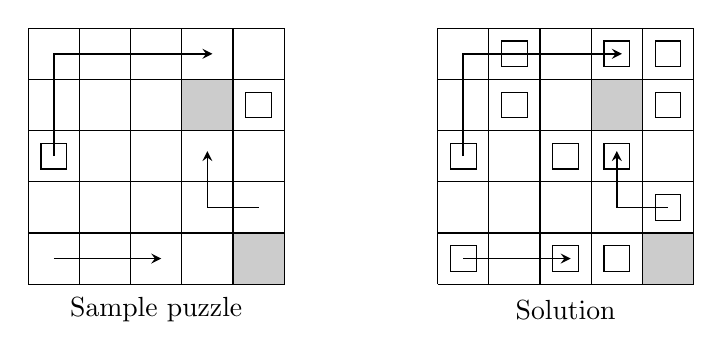
\begin{tikzpicture}[scale=0.65]
			
			\foreach \x in {0,...,5}
			\draw (\x+0.5,0.5)--(\x+0.5,5.5);
			
			\foreach \y in {0,...,5}
			\draw (0.5,\y+0.5)--(5.5,\y+0.5);
			
			
			\foreach \x in {5}	
			\foreach \y in {1}
			\draw [fill = gray!40] (\x-0.5,\y-0.5) -- (\x+0.5,\y-0.5) -- (\x+0.5,\y+0.5) -- (\x-0.5,\y+0.5) -- cycle;	
			
			\foreach \x in {4}	
			\foreach \y in {4}
			\draw [fill = gray!40] (\x-0.5,\y-0.5) -- (\x+0.5,\y-0.5) -- (\x+0.5,\y+0.5) -- (\x-0.5,\y+0.5) -- cycle;			
			
			
			\draw [semithick,->,>=stealth] (1,1) -- (3+0.1,1);
			\draw [semithick,->,>=stealth] (1,3) -- (1,5) -- (4+0.1,5);
			\draw [semithick,->,>=stealth] (5,2) -- (4,2) -- (4,3+0.1);
			
			\foreach \x in {1}
			\foreach \y in {3}
			\draw (\x-0.25,\y-0.25) -- (\x+0.25,\y-0.25) -- (\x+0.25,\y+0.25) -- (\x-0.25,\y+0.25) -- cycle;
			
			
			\foreach \x in {5}
			\foreach \y in {4}
			\draw (\x-0.25,\y-0.25) -- (\x+0.25,\y-0.25) -- (\x+0.25,\y+0.25) -- (\x-0.25,\y+0.25) -- cycle;
			
			\node at (3,0) {Sample puzzle};
			
			\begin{scope}[xshift=8cm]
				
				\foreach \x in {0,...,5}
				\draw (\x+0.5,0.5)--(\x+0.5,5.5);
				
				\foreach \y in {0,...,5}
				\draw (0.5,\y+0.5)--(5.5,\y+0.5);
				
				
				\foreach \x in {5}	
				\foreach \y in {1}
				\draw [fill = gray!40] (\x-0.5,\y-0.5) -- (\x+0.5,\y-0.5) -- (\x+0.5,\y+0.5) -- (\x-0.5,\y+0.5) -- cycle;	
				
				\foreach \x in {4}	
				\foreach \y in {4}
				\draw [fill = gray!40] (\x-0.5,\y-0.5) -- (\x+0.5,\y-0.5) -- (\x+0.5,\y+0.5) -- (\x-0.5,\y+0.5) -- cycle;			
				
				
				\draw [semithick,->,>=stealth] (1,1) -- (3+0.1,1);
				\draw [semithick,->,>=stealth] (1,3) -- (1,5) -- (4+0.1,5);
				\draw [semithick,->,>=stealth] (5,2) -- (4,2) -- (4,3+0.1);
				
				\foreach \x in {1}
				\foreach \y in {1,3}
				\draw (\x-0.25,\y-0.25) -- (\x+0.25,\y-0.25) -- (\x+0.25,\y+0.25) -- (\x-0.25,\y+0.25) -- cycle;
				
				\foreach \x in {2}
				\foreach \y in {4,5}
				\draw (\x-0.25,\y-0.25) -- (\x+0.25,\y-0.25) -- (\x+0.25,\y+0.25) -- (\x-0.25,\y+0.25) -- cycle;
				
				\foreach \x in {3}
				\foreach \y in {1,3}
				\draw (\x-0.25,\y-0.25) -- (\x+0.25,\y-0.25) -- (\x+0.25,\y+0.25) -- (\x-0.25,\y+0.25) -- cycle;
				
				\foreach \x in {4}
				\foreach \y in {1,3,5}
				\draw (\x-0.25,\y-0.25) -- (\x+0.25,\y-0.25) -- (\x+0.25,\y+0.25) -- (\x-0.25,\y+0.25) -- cycle;
				
				\foreach \x in {5}
				\foreach \y in {2,4,5}
				\draw (\x-0.25,\y-0.25) -- (\x+0.25,\y-0.25) -- (\x+0.25,\y+0.25) -- (\x-0.25,\y+0.25) -- cycle;
				
				\node at (3,0) {Solution};
			\end{scope}
		\end{tikzpicture}
		\caption {Example of Evolomino puzzle}
		\label {Fig_Evolomino_example}
	\end{figure}
	
	
	The study of the computational complexity of various games and puzzles is a rapidly growing area of theoretical computer science.
	There are several reasons for this. 
	On the one hand, from an academic and educational point of view, games and puzzles provide a more interesting version of combinatorial problems for learning computational complexity proofs and techniques.
	On the other hand, knowledge of the complexity of a problem helps in developing algorithms for solving puzzles and constructing winning strategies in combinatorial games with two or more players.
	
	Many classic games are known to be computationally intractable (assuming P $\neq$ NP): one-player puzzles are often NP-complete (as Minesweeper~\cite{Kaye2000}, Plumber~\cite{Kral2004}, and Tetris~\cite{Breukelaar2004}) or PSPACE-complete (as Rush Hour~\cite{Flake2002}), and two-player games are often PSPACE-complete (as Hex~\cite{Reisch1981} and Reversi~\cite{Iwata1994}) or EXPTIME-complete (as Chess~\cite{Frankel1981} and Go~\cite{Robson1983}).
	
	In particular, many pencil-and-paper logic puzzles introduced or popularized by Nikoli are NP-complete: Sudoku~\cite{Yato2003}, Kakuro~\cite{Ruepp2010,Seta2002}, Hashiwokakero~\cite{Anderson2009}, Numberlink~\cite{Kotsuma2010}, Shikaku and Ripple effect~\cite{Yasuhiko2013}, Shakashaka~\cite{Demaine2014}, and many others. 
	For more results on the computational complexity of games and puzzles, see the surveys by Demaine and Hearn~\cite{Demaine2009} and Kendall et al.~\cite{Kendall2008}.
	
	In this paper, we prove that the question of whether there exists at least one solution of Evolomino puzzle is also an NP-complete problem by reduction from \textsc{3-SAT}.
	Because our reduction preserves the number of solutions, we also prove that counting the number of solutions to an Evolomino puzzle is $\texttt{\#}$P-complete.
	
	
	\section{Problem statement}
	
	Let us begin with a formal definition of the Evolomino puzzle.
	
	\vspace{2mm}
	
	\textbf{\textsc{Evolomino.}}
	
	\textsc{Instance.} Given a rectangular board of size $p \times q$. Each cell is colored either white or black. Some white cells contain pre-drawn squares ($\square$). The board also contains pre-drawn arrows. Each arrow starts at the center of one cell and ends at the center of another, passing through the centers of the cells on its way horizontally, vertically, or turning 90 degrees. Two arrows cannot occupy the same cell.
	
	\textsc{Question.} 
	Is there at least one solution to the puzzle, i.e., a mapping from the set of white cells to the set $\{\emptyset, \square\}$ that satisfies the rules of the puzzle (each block contains exactly one square placed on the arrow, each arrow passes through at least two blocks, the sizes of the blocks increase in the direction of the arrow, maintaining the shape)?
	
	\vspace{2mm}
	
	We also consider a problem of \textsc{Counting Evolomino}, which has the same instance but asks how many distinct solutions the puzzle has.
	
	
	\section{Evolomino $\in$ NP}
	
	\begin{lemma}
		\textsc{Evolomino} $\in$ NP. \label{Lemma_Evolomino_in_NP}
	\end{lemma}
	
	\begin{proof}
		\textsc{Evolomino} is a decision problem, which means that to prove that it belongs to the class NP, it is sufficient to show that verifying that a given solution satisfies all the rules of the puzzle is performed in polynomial time.
		
		Let us be given an \textsc{Evolomino} puzzle on a rectangular board of size $p \times q$. If we guess some solution to the puzzle, then checking its correctness will require:
		
		\begin{itemize}
			\item Rule: ``Each block must contain exactly one square placed on a pre-drawn arrow.'' 
			
			Since each board cell can belong to no more than one block, we have at most $O(pq)$ blocks. The complexity of traversing one block is linear in its size, which does not exceed the size of $p \times q$ of the entire board. Thus, the total complexity of verifying this rule is $O(p^2 q^2)$.
			
			\item Rule: ``Each arrow must pass through at least two blocks''.
			
			Checking this rule requires a single pass through each pre-drawn arrow. Since the total length of all arrows does not exceed the size of the entire board, the complexity of verifying the rule is $O(pq)$.
			
			\item Rule: ``The second and later blocks on the route of an arrow from start to finish must progress by adding one square to the previous block without rotating or flipping''.
			
			Let us consider two consecutive blocks in the direction of the arrow, both of size no greater than $O(pq)$. Let's try to exclude each square of the second block one by one, after which it remains to go through both blocks and check that they coincide. Therefore, the complexity of verifying the rule for two consecutive blocks does not exceed $O(p^2 q^2)$.
			
			It remains to note that the number of pairs of consecutive blocks does not exceed the total length of all pre-drawn arrows, i.e., $O(pq)$. Which makes the overall complexity of verifying the rule equal to $O(p^3 q^3)$.
		\end{itemize}
		
		Summing up the complexity of all the rules, we find that a given puzzle solution can be verified in polynomial time $O(p^3 q^3)$. Note that this is a fairly rough estimate, but to prove that \textsc{Evolomino} $\in$ NP, it is sufficient to be polynomial in the size of the board $p \times q$.
	\end{proof}
	
	
	
	\section{Evolomino is NP-complete}
	
	\begin{theorem}
		\textsc{Evolomino} is NP-complete.
	\end{theorem}
	
	\begin{proof}

	To prove that \textsc{Evolomino} is NP-hard, we construct a polynomial-time reduction from NP-complete \textsc{3-SAT} problem~\cite{Garey1979,Karp1972} to \textsc{Evolomino}.
	
	\vspace{2mm}
	
	\textbf{\textsc{3-SAT.}}
	
	\textsc{Instance.} Given a Boolean formula in conjunctive normal form (CNF), i.e., a collection $C = \{C_1,\ldots,C_m\}$ of clauses on a finite set $X=\{x_1,\ldots,x_n\}$ of Boolean variables such that $|C_i| = 3$ for all $1 \leq i \leq m$.
	
	\textsc{Question.} Is there a truth assignment for variables $X$ that satisfies all the clauses in $C$, and therefore satisfy the Boolean formula?	
	
	\vspace{2mm}
	
	We model each component of \textsc{3-SAT} with some gadgets on the \textsc{Evolomino} board so that the puzzle has a solution if and only if the corresponding instance of \textsc{3-SAT} is satisfiable.
	
	
	\subsubsection{Variable and wire gadget.}
	
	The variable and wire gadget models the truth assignment to a Boolean variable. Its structure is shown in Fig.~\ref{Fig_variable_wire_gadget}.
	
	Since each block must contain exactly one square placed on an arrow and each subsequent block on the route of an arrow must progress by adding one square to the previous block without rotating or flipping, there are only two options to correctly place the squares in the solution: Fig.~\ref{Fig_variable_wire_gadget} (a) that corresponds for $x = 1$ and Fig.~\ref{Fig_variable_wire_gadget} (b) for $x = 0$.
	
	\begin{figure}[t]
	\centering
		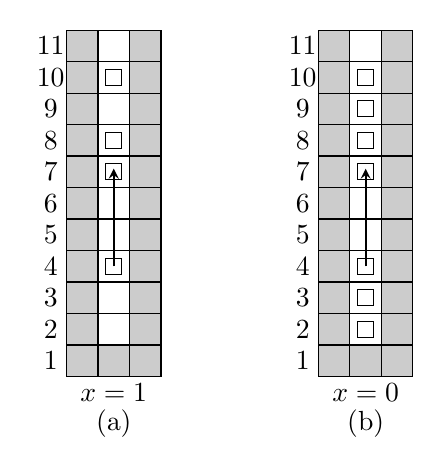
\begin{tikzpicture}[scale=0.40]
		
			\foreach \y in {1,...,11}
				\node at (0,\y) {\y};
			
			\node at (2,0) {$x=1$};
			
			\node at (2,-1) {(a)};
			
			\foreach \x in {0,...,3}
			\draw (\x+0.5,0.5)--(\x+0.5,11.5);
			
			\foreach \y in {0,...,11}
			\draw (0.5,\y+0.5)--(3.5,\y+0.5);
			
			\foreach \x in {1,3}	
			\foreach \y in {1,...,11}
			\draw [fill = gray!40] (\x-0.5,\y-0.5) -- (\x+0.5,\y-0.5) -- (\x+0.5,\y+0.5) -- (\x-0.5,\y+0.5) -- cycle;	
			
			\foreach \x in {2}	
			\foreach \y in {1}
			\draw [fill = gray!40] (\x-0.5,\y-0.5) -- (\x+0.5,\y-0.5) -- (\x+0.5,\y+0.5) -- (\x-0.5,\y+0.5) -- cycle;	
			
			\foreach \x in {2}
			\foreach \y in {4,7,8,10}
			\draw (\x-0.25,\y-0.25) -- (\x+0.25,\y-0.25) -- (\x+0.25,\y+0.25) -- (\x-0.25,\y+0.25) -- cycle;
			
			\draw [semithick,->,>=stealth] (2,4) -- (2,7+0.1);
			
			
			\begin{scope}[xshift=8cm]
				
				\foreach \y in {1,...,11}
					\node at (0,\y) {\y};
				
				\node at (2,0) {$x=0$};
				
				\node at (2,-1) {(b)};
				
				\foreach \x in {0,...,3}
				\draw (\x+0.5,0.5)--(\x+0.5,11.5);
				
				\foreach \y in {0,...,11}
				\draw (0.5,\y+0.5)--(3.5,\y+0.5);
				
				\foreach \x in {1,3}	
				\foreach \y in {1,...,11}
				\draw [fill = gray!40] (\x-0.5,\y-0.5) -- (\x+0.5,\y-0.5) -- (\x+0.5,\y+0.5) -- (\x-0.5,\y+0.5) -- cycle;	
				
				\foreach \x in {2}	
				\foreach \y in {1}
				\draw [fill = gray!40] (\x-0.5,\y-0.5) -- (\x+0.5,\y-0.5) -- (\x+0.5,\y+0.5) -- (\x-0.5,\y+0.5) -- cycle;	
				
				\foreach \x in {2}
				\foreach \y in {2,3,4,7,8,9,10}
				\draw (\x-0.25,\y-0.25) -- (\x+0.25,\y-0.25) -- (\x+0.25,\y+0.25) -- (\x-0.25,\y+0.25) -- cycle;
				
				\draw [semithick,->,>=stealth] (2,4) -- (2,7+0.1);
			\end{scope}
		\end{tikzpicture}
		\caption {Variable and wire gadget}
		\label {Fig_variable_wire_gadget}
	\end{figure}
	
	The encoding in which 1 square is 1 and 3 squares is 0 may seem a bit counter-intuitive, but it will be explained further in the clause gadget. We interpret 1 as an open lock and 0 as a closed lock.
	
	The arrow itself acts as a wire gadget, transmitting the signal from start to finish. To ensure the signal is not disrupted by other possible blocks, we fence each arrow on both sides with black cells.
	
	
	\subsubsection{Negation gadget.}
	
	The negation gadget that inverts the value of a Boolean variable
	is shown in Fig.~\ref{Fig_negation_gadget} (a).
	It consists of two variable gadgets with a single square between them.
	Since one of the squares of each block must be placed on the arrow, then this square in the solution will be included either in one block Fig.~\ref{Fig_negation_gadget} (b), or in another Fig.~\ref{Fig_negation_gadget} (c), which ensures the inversion of the signal.
	
	\begin{figure}[p]
		\centering
		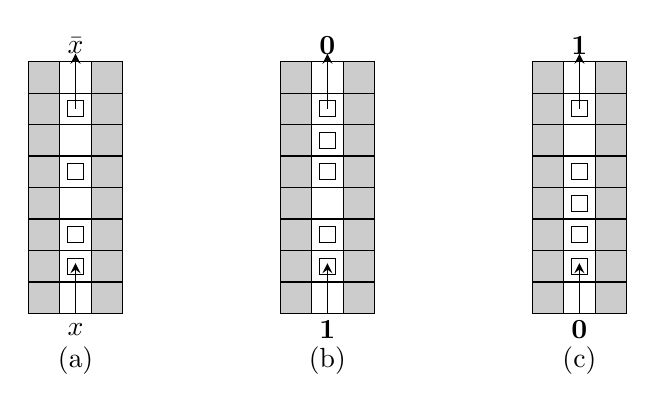
\begin{tikzpicture}[scale=0.40]
			
		%	\foreach \y in {1,...,8}
		%		\node at (0,\y) {\y};
			
			\foreach \x in {0,...,3}
			\draw (\x+0.5,0.5)--(\x+0.5,8.5);
			
			\foreach \y in {0,...,8}
			\draw (0.5,\y+0.5)--(3.5,\y+0.5);
			
			\foreach \x in {1,3}	
			\foreach \y in {1,...,8}
			\draw [fill = gray!40] (\x-0.5,\y-0.5) -- (\x+0.5,\y-0.5) -- (\x+0.5,\y+0.5) -- (\x-0.5,\y+0.5) -- cycle;	
			
				
			\foreach \x in {2}
			\foreach \y in {2,3,5,7}
			\draw (\x-0.25,\y-0.25) -- (\x+0.25,\y-0.25) -- (\x+0.25,\y+0.25) -- (\x-0.25,\y+0.25) -- cycle;
			
			\draw [semithick,->,>=stealth] (2,0.5) -- (2,2+0.1);
			\draw [semithick,->,>=stealth] (2,7) -- (2,8+0.75);
			
			\node at (2,0) {$x$};
			\node at (2,9) {$\bar{x}$};
			
			\node at (2,-1) {(a)};
			
			\begin{scope}[xshift=8cm]
				
		%		\foreach \y in {1,...,8}
		%		\node at (0,\y) {\y};
				
				\foreach \x in {0,...,3}
				\draw (\x+0.5,0.5)--(\x+0.5,8.5);
				
				\foreach \y in {0,...,8}
				\draw (0.5,\y+0.5)--(3.5,\y+0.5);
				
				\foreach \x in {1,3}	
				\foreach \y in {1,...,8}
				\draw [fill = gray!40] (\x-0.5,\y-0.5) -- 	(\x+0.5,\y-0.5) -- (\x+0.5,\y+0.5) -- (\x-0.5,\y+0.5) -- cycle;	
				
				
				\foreach \x in {2}
				\foreach \y in {2,3,5,6,7}
				\draw (\x-0.25,\y-0.25) -- (\x+0.25,\y-0.25) -- 	(\x+0.25,\y+0.25) -- (\x-0.25,\y+0.25) -- cycle;
				
				\draw [semithick,->,>=stealth] (2,0.5) -- (2,2+0.1);
				\draw [semithick,->,>=stealth] (2,7) -- (2,8+0.75);
				
				\node at (2,0) {\bf{1}};	
				\node at (2,9) {\bf{0}};
				
				\node at (2,-1) {(b)};
			
			\end{scope}
			
			\begin{scope}[xshift=16cm]
				
		%		\foreach \y in {1,...,8}
		%		\node at (0,\y) {\y};
				
				\foreach \x in {0,...,3}
				\draw (\x+0.5,0.5)--(\x+0.5,8.5);
				
				\foreach \y in {0,...,8}
				\draw (0.5,\y+0.5)--(3.5,\y+0.5);
				
				\foreach \x in {1,3}	
				\foreach \y in {1,...,8}
				\draw [fill = gray!40] (\x-0.5,\y-0.5) -- (\x+0.5,\y-0.5) -- (\x+0.5,\y+0.5) -- (\x-0.5,\y+0.5) -- cycle;	
				
				
				\foreach \x in {2}
				\foreach \y in {2,3,4,5,7}
				\draw (\x-0.25,\y-0.25) -- (\x+0.25,\y-0.25) -- (\x+0.25,\y+0.25) -- (\x-0.25,\y+0.25) -- cycle;
				
				\draw [semithick,->,>=stealth] (2,0.5) -- (2,2+0.1);
				\draw [semithick,->,>=stealth] (2,7) -- (2,8+0.75);
				
				\node at (2,0) {\bf{0}};	
				\node at (2,9) {\bf{1}};
				
				\node at (2,-1) {(c)};
				
			\end{scope}
		\end{tikzpicture}
		\caption {Negation gadget}
		\label {Fig_negation_gadget}
	\end{figure}
	
	
	\subsubsection{Split gadget.}
	
	The split gadget shown in Fig.~\ref{Fig_split_gadget} (a) is needed for signal duplication when one variable is included in several clauses.
	
	Again, given that each block must be placed on an arrow and the block shape is inherited in the direction of the arrow without rotating and flipping, there are only 2 feasible solutions to the puzzle: Fig.~\ref{Fig_split_gadget} (b) for splitting the $x=1$ signal and Fig.~\ref{Fig_split_gadget} (c) for $x=0$.
	
	\begin{figure}[p]
		\centering
		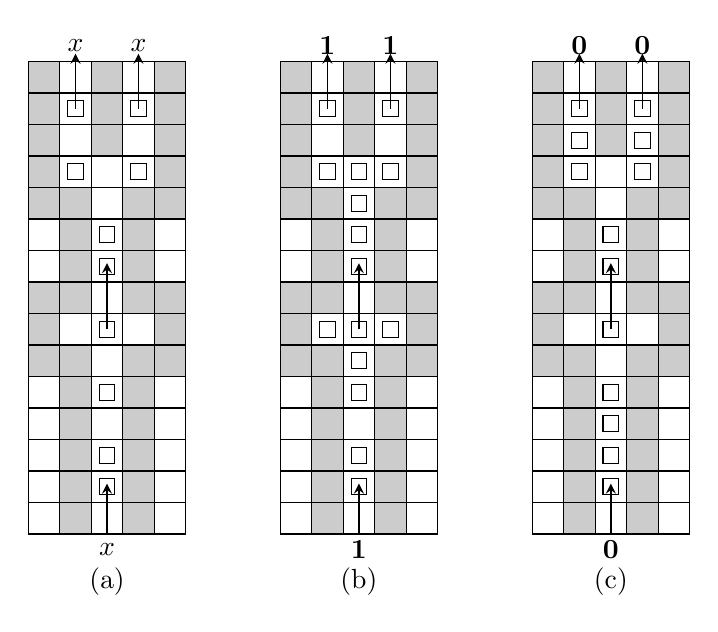
\begin{tikzpicture}[scale=0.40]
			
		%	\foreach \y in {1,...,15}
		%		\node at (0,\y) {\y};
			
			\node at (3,-1) {(a)};
			
			\node at (3,0) {$x$};
			\node at (2,16) {$x$};
			\node at (4,16) {$x$};
			
			\foreach \x in {0,...,5}
			\draw (\x+0.5,0.5)--(\x+0.5,15.5);
			
			\foreach \y in {0,...,15}
			\draw (0.5,\y+0.5)--(5.5,\y+0.5);
			
			\foreach \x in {2,4}	
			\foreach \y in {1,...,6,8,9,10,11}
			\draw [fill = gray!40] (\x-0.5,\y-0.5) -- (\x+0.5,\y-0.5) -- (\x+0.5,\y+0.5) -- (\x-0.5,\y+0.5) -- cycle;	
			
			\foreach \x in {1,5}	
			\foreach \y in {6,7,8,11,12,...,15}
			\draw [fill = gray!40] (\x-0.5,\y-0.5) -- (\x+0.5,\y-0.5) -- (\x+0.5,\y+0.5) -- (\x-0.5,\y+0.5) -- cycle;	
			
			\foreach \x in {3}	
			\foreach \y in {13,...,15}
			\draw [fill = gray!40] (\x-0.5,\y-0.5) -- (\x+0.5,\y-0.5) -- (\x+0.5,\y+0.5) -- (\x-0.5,\y+0.5) -- cycle;	
			
			\foreach \x in {3}
			\foreach \y in {2,3,5,7,9,10}
			\draw (\x-0.25,\y-0.25) -- (\x+0.25,\y-0.25) -- (\x+0.25,\y+0.25) -- (\x-0.25,\y+0.25) -- cycle;
			
			\foreach \x in {2,4}
			\foreach \y in {12,14}
			\draw (\x-0.25,\y-0.25) -- (\x+0.25,\y-0.25) -- (\x+0.25,\y+0.25) -- (\x-0.25,\y+0.25) -- cycle;
			
			\draw [semithick,->,>=stealth] (3,0.5) -- (3,2+0.1);
			\draw [semithick,->,>=stealth] (3,7) -- (3,9+0.1);
			\draw [semithick,->,>=stealth] (2,14) -- (2,15+0.75);
			\draw [semithick,->,>=stealth] (4,14) -- (4,15+0.75);
			
			
			\begin{scope}[xshift=8cm]
		%		\foreach \y in {1,...,15}
		%			\node at (0,\y) {\y};
				
				\node at (3,-1) {(b)};
				
				\node at (3,0) {\bf{1}};
				\node at (2,16) {\bf{1}};
				\node at (4,16) {\bf{1}};
				
				\foreach \x in {0,...,5}
				\draw (\x+0.5,0.5)--(\x+0.5,15.5);
				
				\foreach \y in {0,...,15}
				\draw (0.5,\y+0.5)--(5.5,\y+0.5);
				
				\foreach \x in {2,4}	
				\foreach \y in {1,...,6,8,9,10,11}
				\draw [fill = gray!40] (\x-0.5,\y-0.5) -- (\x+0.5,\y-0.5) -- (\x+0.5,\y+0.5) -- (\x-0.5,\y+0.5) -- cycle;	
				
				\foreach \x in {1,5}	
				\foreach \y in {6,7,8,11,12,...,15}
				\draw [fill = gray!40] (\x-0.5,\y-0.5) -- (\x+0.5,\y-0.5) -- (\x+0.5,\y+0.5) -- (\x-0.5,\y+0.5) -- cycle;	
				
				\foreach \x in {3}	
				\foreach \y in {13,...,15}
				\draw [fill = gray!40] (\x-0.5,\y-0.5) -- (\x+0.5,\y-0.5) -- (\x+0.5,\y+0.5) -- (\x-0.5,\y+0.5) -- cycle;	
				
				\foreach \x in {3}
				\foreach \y in {2,3,5,6,7,9,10,11,12}
				\draw (\x-0.25,\y-0.25) -- (\x+0.25,\y-0.25) -- (\x+0.25,\y+0.25) -- (\x-0.25,\y+0.25) -- cycle;			
				
				
				\foreach \x in {2,4}
				\foreach \y in {7,12,14}
				\draw (\x-0.25,\y-0.25) -- (\x+0.25,\y-0.25) -- (\x+0.25,\y+0.25) -- (\x-0.25,\y+0.25) -- cycle;
				
				\draw [semithick,->,>=stealth] (3,0.5) -- (3,2+0.1);
				\draw [semithick,->,>=stealth] (3,7) -- (3,9+0.1);
				\draw [semithick,->,>=stealth] (2,14) -- (2,15+0.75);
				\draw [semithick,->,>=stealth] (4,14) -- (4,15+0.75);
			\end{scope}
			
			\begin{scope}[xshift=16cm]
		%		\foreach \y in {1,...,15}
		%			\node at (0,\y) {\y};
				
				\node at (3,-1) {(c)};
				
				\node at (3,0) {\bf {0}};
				\node at (2,16) {\bf{0}};
				\node at (4,16) {\bf{0}};
				
				\foreach \x in {0,...,5}
				\draw (\x+0.5,0.5)--(\x+0.5,15.5);
				
				\foreach \y in {0,...,15}
				\draw (0.5,\y+0.5)--(5.5,\y+0.5);
				
				\foreach \x in {2,4}	
				\foreach \y in {1,...,6,8,9,10,11}
				\draw [fill = gray!40] (\x-0.5,\y-0.5) -- 	(\x+0.5,\y-0.5) -- (\x+0.5,\y+0.5) -- (\x-0.5,\y+0.5) -- cycle;	
				
				\foreach \x in {1,5}	
				\foreach \y in {6,7,8,11,12,...,15}
				\draw [fill = gray!40] (\x-0.5,\y-0.5) -- 	(\x+0.5,\y-0.5) -- (\x+0.5,\y+0.5) -- (\x-0.5,\y+0.5) -- cycle;	
				
				\foreach \x in {3}	
				\foreach \y in {13,...,15}
				\draw [fill = gray!40] (\x-0.5,\y-0.5) -- 	(\x+0.5,\y-0.5) -- (\x+0.5,\y+0.5) -- (\x-0.5,\y+0.5) -- cycle;	
				
				\foreach \x in {3}
				\foreach \y in {2,3,4,5,7,9,10}
				\draw (\x-0.25,\y-0.25) -- (\x+0.25,\y-0.25) -- 	(\x+0.25,\y+0.25) -- (\x-0.25,\y+0.25) -- cycle;
				
				\foreach \x in {2,4}
				\foreach \y in {12,13,14}
				\draw (\x-0.25,\y-0.25) -- (\x+0.25,\y-0.25) -- 	(\x+0.25,\y+0.25) -- (\x-0.25,\y+0.25) -- cycle;
				
				\draw [semithick,->,>=stealth] (3,0.5) -- (3,2+0.1);
				\draw [semithick,->,>=stealth] (3,7) -- (3,9+0.1);
				\draw [semithick,->,>=stealth] (2,14) -- (2,15+0.75);
				\draw [semithick,->,>=stealth] (4,14) -- (4,15+0.75);
				\end{scope}
		\end{tikzpicture}
		\caption {Split gadget}
		\label {Fig_split_gadget}
	\end{figure}
	
	\subsubsection{Clause gadget.}
	
	The structure of the clause gadget for a clause $C=\{x \vee y\vee z\}$ is shown in Fig.~\ref{Fig_clause_gadget}. Since there is a vertical line block of 5 squares at the end of the horizontal arrow, according to the rules of the puzzle it must be preceded by a vertical line block of 4 squares.
	It is easy to see that such a block can only be placed in one of the three columns corresponding to the literals $x$, $y$, and $z$.
	However, if a false signal is received in the literal, then the corresponding column is locked since a block of squares cannot be placed on two different arrows at the same time.
	Thus, the puzzle in the clause gadget has a solution if and only if at least one of the literals $x$, $y$, or $z$ is satisfied.
	An example of three feasible cases (a), (b), (c) and one infeasible case (d) of a clause gadget is shown in Fig.~\ref{Fig_clause_gadget_feasible}.
	
	\begin{figure}[p]
		\centering
		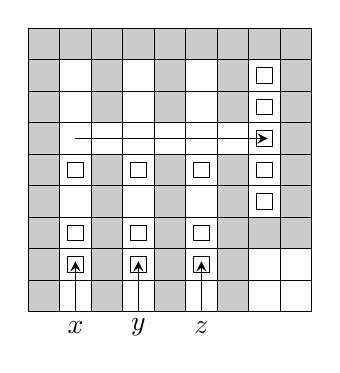
\begin{tikzpicture}[scale=0.40]
			
	%		\foreach \y in {1,...,9}
	%		\node at (0,\y) {\y};
			
	%		\foreach \x in {1,...,9}
	%		\node at (\x,10) {\x};
			
			\foreach \x in {0,...,9}
			\draw (\x+0.5,0.5)--(\x+0.5,9.5);
			
			\foreach \y in {0,...,9}
			\draw (0.5,\y+0.5)--(9.5,\y+0.5);
			
			\foreach \x in {1}	
			\foreach \y in {1,...,9}
			\draw [fill = gray!40] (\x-0.5,\y-0.5) -- (\x+0.5,\y-0.5) -- (\x+0.5,\y+0.5) -- (\x-0.5,\y+0.5) -- cycle;	
			
			\foreach \x in {3,5,7}	
			\foreach \y in {1,...,5,7,8,9}
			\draw [fill = gray!40] (\x-0.5,\y-0.5) -- (\x+0.5,\y-0.5) -- (\x+0.5,\y+0.5) -- (\x-0.5,\y+0.5) -- cycle;	
			
			\foreach \x in {2,4,6}	
			\foreach \y in {9}
			\draw [fill = gray!40] (\x-0.5,\y-0.5) -- (\x+0.5,\y-0.5) -- (\x+0.5,\y+0.5) -- (\x-0.5,\y+0.5) -- cycle;	
			
			\foreach \x in {8}	
			\foreach \y in {3,9}
			\draw [fill = gray!40] (\x-0.5,\y-0.5) -- (\x+0.5,\y-0.5) -- (\x+0.5,\y+0.5) -- (\x-0.5,\y+0.5) -- cycle;	
			
			\foreach \x in {9}	
			\foreach \y in {3,...,9}
			\draw [fill = gray!40] (\x-0.5,\y-0.5) -- (\x+0.5,\y-0.5) -- (\x+0.5,\y+0.5) -- (\x-0.5,\y+0.5) -- cycle;	
			
			
			\foreach \x in {2,4,6}
			\foreach \y in {2,3,5}
			\draw (\x-0.25,\y-0.25) -- (\x+0.25,\y-0.25) -- (\x+0.25,\y+0.25) -- (\x-0.25,\y+0.25) -- cycle;
			
			\foreach \x in {8}
			\foreach \y in {4,...,8}
			\draw (\x-0.25,\y-0.25) -- (\x+0.25,\y-0.25) -- (\x+0.25,\y+0.25) -- (\x-0.25,\y+0.25) -- cycle;
			
			\draw [semithick,->,>=stealth] (2,6) -- (8+0.1,6);
			
			\foreach \x in {2,4,6}
			\draw [semithick,->,>=stealth] (\x,0.5) -- (\x,2+0.1);
			
			\node at (2,0) {$x$};
			\node at (4,0) {$y$};
			\node at (6,0) {$z$};
			
		\end{tikzpicture}
		\caption {Clause gadget}
		\label {Fig_clause_gadget}
	\end{figure}
	
	
	\begin{figure}[p]
		\centering
		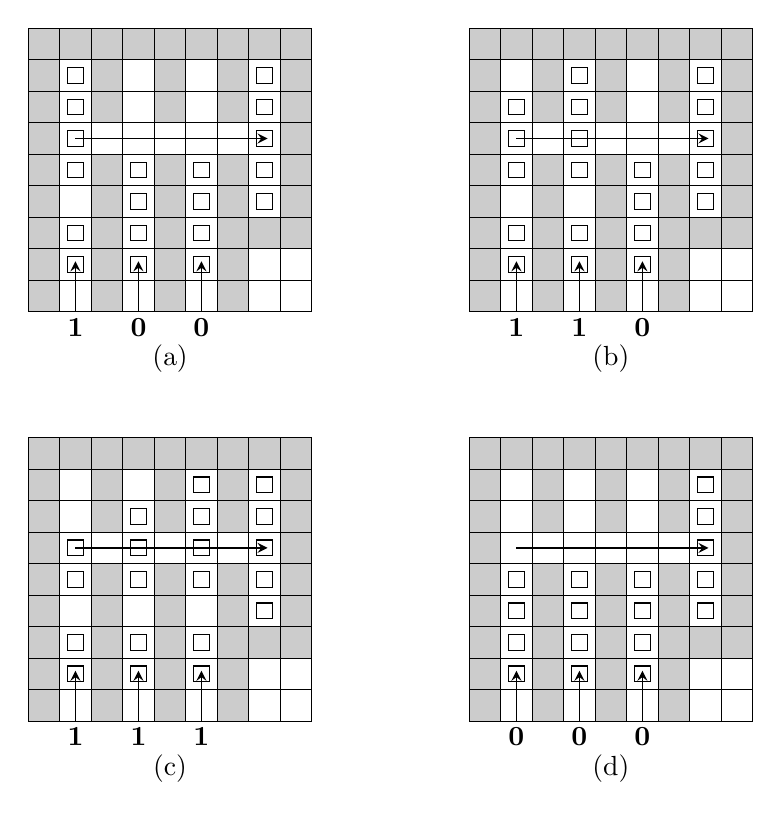
\begin{tikzpicture}[scale=0.40]
			
		%	\foreach \y in {1,...,9}
		%	\node at (0,\y) {\y};
			
		%	\foreach \x in {1,...,9}
		%	\node at (\x,10) {\x};
			
			\foreach \x in {0,...,9}
			\draw (\x+0.5,0.5)--(\x+0.5,9.5);
			
			\foreach \y in {0,...,9}
			\draw (0.5,\y+0.5)--(9.5,\y+0.5);
			
			\foreach \x in {1}	
			\foreach \y in {1,...,9}
			\draw [fill = gray!40] (\x-0.5,\y-0.5) -- (\x+0.5,\y-0.5) -- (\x+0.5,\y+0.5) -- (\x-0.5,\y+0.5) -- cycle;	
			
			\foreach \x in {3,5,7}	
			\foreach \y in {1,...,5,7,8,9}
			\draw [fill = gray!40] (\x-0.5,\y-0.5) -- (\x+0.5,\y-0.5) -- (\x+0.5,\y+0.5) -- (\x-0.5,\y+0.5) -- cycle;	
			
			\foreach \x in {2,4,6}	
			\foreach \y in {9}
			\draw [fill = gray!40] (\x-0.5,\y-0.5) -- (\x+0.5,\y-0.5) -- (\x+0.5,\y+0.5) -- (\x-0.5,\y+0.5) -- cycle;	
			
			\foreach \x in {8}	
			\foreach \y in {3,9}
			\draw [fill = gray!40] (\x-0.5,\y-0.5) -- (\x+0.5,\y-0.5) -- (\x+0.5,\y+0.5) -- (\x-0.5,\y+0.5) -- cycle;	
			
			\foreach \x in {9}	
			\foreach \y in {3,...,9}
			\draw [fill = gray!40] (\x-0.5,\y-0.5) -- (\x+0.5,\y-0.5) -- (\x+0.5,\y+0.5) -- (\x-0.5,\y+0.5) -- cycle;	
			
			
			\foreach \x in {2}
			\foreach \y in {2,3,5,6,7,8}
			\draw (\x-0.25,\y-0.25) -- (\x+0.25,\y-0.25) -- (\x+0.25,\y+0.25) -- (\x-0.25,\y+0.25) -- cycle;
			
			\foreach \x in {4,6}
			\foreach \y in {2,3,4,5}
			\draw (\x-0.25,\y-0.25) -- (\x+0.25,\y-0.25) -- (\x+0.25,\y+0.25) -- (\x-0.25,\y+0.25) -- cycle;
			
			\foreach \x in {8}
			\foreach \y in {4,...,8}
			\draw (\x-0.25,\y-0.25) -- (\x+0.25,\y-0.25) -- (\x+0.25,\y+0.25) -- (\x-0.25,\y+0.25) -- cycle;
			
			\draw [semithick,->,>=stealth] (2,6) -- (8+0.1,6);
			
			\foreach \x in {2,4,6}
			\draw [semithick,->,>=stealth] (\x,0.5) -- (\x,2+0.1);
			
			\node at (2,0) {\bf{1}};
			\node at (4,0) {\bf{0}};
			\node at (6,0) {\bf{0}};
			
			\node at (5,-1) {(a)};
			
			
			\begin{scope}[xshift=14cm]
		%		\foreach \y in {1,...,9}
		%		\node at (0,\y) {\y};
				
		%		\foreach \x in {1,...,9}
		%		\node at (\x,10) {\x};
				
				\foreach \x in {0,...,9}
				\draw (\x+0.5,0.5)--(\x+0.5,9.5);
				
				\foreach \y in {0,...,9}
				\draw (0.5,\y+0.5)--(9.5,\y+0.5);
				
				\foreach \x in {1}	
				\foreach \y in {1,...,9}
				\draw [fill = gray!40] (\x-0.5,\y-0.5) -- (\x+0.5,\y-0.5) -- (\x+0.5,\y+0.5) -- (\x-0.5,\y+0.5) -- cycle;	
				
				\foreach \x in {3,5,7}	
				\foreach \y in {1,...,5,7,8,9}
				\draw [fill = gray!40] (\x-0.5,\y-0.5) -- (\x+0.5,\y-0.5) -- (\x+0.5,\y+0.5) -- (\x-0.5,\y+0.5) -- cycle;	
				
				\foreach \x in {2,4,6}	
				\foreach \y in {9}
				\draw [fill = gray!40] (\x-0.5,\y-0.5) -- (\x+0.5,\y-0.5) -- (\x+0.5,\y+0.5) -- (\x-0.5,\y+0.5) -- cycle;	
				
				\foreach \x in {8}	
				\foreach \y in {3,9}
				\draw [fill = gray!40] (\x-0.5,\y-0.5) -- (\x+0.5,\y-0.5) -- (\x+0.5,\y+0.5) -- (\x-0.5,\y+0.5) -- cycle;	
				
				\foreach \x in {9}	
				\foreach \y in {3,...,9}
				\draw [fill = gray!40] (\x-0.5,\y-0.5) -- (\x+0.5,\y-0.5) -- (\x+0.5,\y+0.5) -- (\x-0.5,\y+0.5) -- cycle;	
				
				\foreach \x in {2}
				\foreach \y in {2,3,5,6,7}
				\draw (\x-0.25,\y-0.25) -- (\x+0.25,\y-0.25) -- (\x+0.25,\y+0.25) -- (\x-0.25,\y+0.25) -- cycle;
				
				\foreach \x in {4}
				\foreach \y in {2,3,5,6,7,8}
				\draw (\x-0.25,\y-0.25) -- (\x+0.25,\y-0.25) -- (\x+0.25,\y+0.25) -- (\x-0.25,\y+0.25) -- cycle;
				
				\foreach \x in {6}
				\foreach \y in {2,3,4,5}
				\draw (\x-0.25,\y-0.25) -- (\x+0.25,\y-0.25) -- (\x+0.25,\y+0.25) -- (\x-0.25,\y+0.25) -- cycle;
				
				\foreach \x in {8}
				\foreach \y in {4,...,8}
				\draw (\x-0.25,\y-0.25) -- (\x+0.25,\y-0.25) -- (\x+0.25,\y+0.25) -- (\x-0.25,\y+0.25) -- cycle;
				
				\draw [semithick,->,>=stealth] (2,6) -- (8+0.1,6);
				
				\foreach \x in {2,4,6}
				\draw [semithick,->,>=stealth] (\x,0.5) -- (\x,2+0.1);
				
				\node at (2,0) {\bf{1}};
				\node at (4,0) {\bf{1}};
				\node at (6,0) {\bf{0}};
				
				\node at (5,-1) {(b)};
			\end{scope}
			
			
			\begin{scope}[yshift=-13cm]
		%		\foreach \y in {1,...,9}
		%		\node at (0,\y) {\y};
				
		%		\foreach \x in {1,...,9}
		%		\node at (\x,10) {\x};
				
				\foreach \x in {0,...,9}
				\draw (\x+0.5,0.5)--(\x+0.5,9.5);
				
				\foreach \y in {0,...,9}
				\draw (0.5,\y+0.5)--(9.5,\y+0.5);
				
				\foreach \x in {1}	
				\foreach \y in {1,...,9}
				\draw [fill = gray!40] (\x-0.5,\y-0.5) -- (\x+0.5,\y-0.5) -- (\x+0.5,\y+0.5) -- (\x-0.5,\y+0.5) -- cycle;	
				
				\foreach \x in {3,5,7}	
				\foreach \y in {1,...,5,7,8,9}
				\draw [fill = gray!40] (\x-0.5,\y-0.5) -- (\x+0.5,\y-0.5) -- (\x+0.5,\y+0.5) -- (\x-0.5,\y+0.5) -- cycle;	
				
				\foreach \x in {2,4,6}	
				\foreach \y in {9}
				\draw [fill = gray!40] (\x-0.5,\y-0.5) -- (\x+0.5,\y-0.5) -- (\x+0.5,\y+0.5) -- (\x-0.5,\y+0.5) -- cycle;	
				
				\foreach \x in {8}	
				\foreach \y in {3,9}
				\draw [fill = gray!40] (\x-0.5,\y-0.5) -- (\x+0.5,\y-0.5) -- (\x+0.5,\y+0.5) -- (\x-0.5,\y+0.5) -- cycle;	
				
				\foreach \x in {9}	
				\foreach \y in {3,...,9}
				\draw [fill = gray!40] (\x-0.5,\y-0.5) -- (\x+0.5,\y-0.5) -- (\x+0.5,\y+0.5) -- (\x-0.5,\y+0.5) -- cycle;	
				
				
				\foreach \x in {2}
				\foreach \y in {2,3,5,6}
				\draw (\x-0.25,\y-0.25) -- (\x+0.25,\y-0.25) -- (\x+0.25,\y+0.25) -- (\x-0.25,\y+0.25) -- cycle;
				
				\foreach \x in {4}
				\foreach \y in {2,3,5,6,7}
				\draw (\x-0.25,\y-0.25) -- (\x+0.25,\y-0.25) -- (\x+0.25,\y+0.25) -- (\x-0.25,\y+0.25) -- cycle;
				
				\foreach \x in {6}
				\foreach \y in {2,3,5,6,7,8}
				\draw (\x-0.25,\y-0.25) -- (\x+0.25,\y-0.25) -- (\x+0.25,\y+0.25) -- (\x-0.25,\y+0.25) -- cycle;
				
				\foreach \x in {8}
				\foreach \y in {4,...,8}
				\draw (\x-0.25,\y-0.25) -- (\x+0.25,\y-0.25) -- (\x+0.25,\y+0.25) -- (\x-0.25,\y+0.25) -- cycle;
				
				\draw [semithick,->,>=stealth] (2,6) -- (8+0.1,6);
				
				\foreach \x in {2,4,6}
				\draw [semithick,->,>=stealth] (\x,0.5) -- (\x,2+0.1);
				
				\node at (2,0) {\bf{1}};
				\node at (4,0) {\bf{1}};
				\node at (6,0) {\bf{1}};
				
				\node at (5,-1) {(c)};
			\end{scope}
			
			
			\begin{scope}[xshift=14cm,yshift=-13cm]
		%		\foreach \y in {1,...,9}
		%		\node at (0,\y) {\y};
				
		%		\foreach \x in {1,...,9}
		%		\node at (\x,10) {\x};
				
				\foreach \x in {0,...,9}
				\draw (\x+0.5,0.5)--(\x+0.5,9.5);
				
				\foreach \y in {0,...,9}
				\draw (0.5,\y+0.5)--(9.5,\y+0.5);
				
				\foreach \x in {1}	
				\foreach \y in {1,...,9}
				\draw [fill = gray!40] (\x-0.5,\y-0.5) -- (\x+0.5,\y-0.5) -- (\x+0.5,\y+0.5) -- (\x-0.5,\y+0.5) -- cycle;	
				
				\foreach \x in {3,5,7}	
				\foreach \y in {1,...,5,7,8,9}
				\draw [fill = gray!40] (\x-0.5,\y-0.5) -- (\x+0.5,\y-0.5) -- (\x+0.5,\y+0.5) -- (\x-0.5,\y+0.5) -- cycle;	
				
				\foreach \x in {2,4,6}	
				\foreach \y in {9}
				\draw [fill = gray!40] (\x-0.5,\y-0.5) -- (\x+0.5,\y-0.5) -- (\x+0.5,\y+0.5) -- (\x-0.5,\y+0.5) -- cycle;	
				
				\foreach \x in {8}	
				\foreach \y in {3,9}
				\draw [fill = gray!40] (\x-0.5,\y-0.5) -- (\x+0.5,\y-0.5) -- (\x+0.5,\y+0.5) -- (\x-0.5,\y+0.5) -- cycle;	
				
				\foreach \x in {9}	
				\foreach \y in {3,...,9}
				\draw [fill = gray!40] (\x-0.5,\y-0.5) -- (\x+0.5,\y-0.5) -- (\x+0.5,\y+0.5) -- (\x-0.5,\y+0.5) -- cycle;	
				
				
				\foreach \x in {2,4,6}
				\foreach \y in {2,3,4,5}
				\draw (\x-0.25,\y-0.25) -- (\x+0.25,\y-0.25) -- (\x+0.25,\y+0.25) -- (\x-0.25,\y+0.25) -- cycle;
				
				\foreach \x in {8}
				\foreach \y in {4,...,8}
				\draw (\x-0.25,\y-0.25) -- (\x+0.25,\y-0.25) -- (\x+0.25,\y+0.25) -- (\x-0.25,\y+0.25) -- cycle;
				
				\draw [semithick,->,>=stealth] (2,6) -- (8+0.1,6);
				
				\foreach \x in {2,4,6}
				\draw [semithick,->,>=stealth] (\x,0.5) -- (\x,2+0.1);
				
				\node at (2,0) {\bf{0}};
				\node at (4,0) {\bf{0}};
				\node at (6,0) {\bf{0}};
				
				\node at (5,-1) {(d)};
			\end{scope}
			
		\end{tikzpicture}
		\caption {Three feasible cases (a), (b), (c) and one infeasible case (d) of a clause gadget}
		\label {Fig_clause_gadget_feasible}
	\end{figure}
	
	
	
	\subsubsection{Crossover gadget.}
	
	Signals coming from variable gadgets to clause gadgets may cross on the way. To solve this problem, we additionally consider the crossover gadget shown in Fig.~\ref{Fig_crossover_gadget}, as well as all 4 of its feasible solutions corresponding to 4 sets of values of crossing signals presented in Fig.~\ref{Fig_crossover_gadget_cases}.
	
	
	
	\begin{figure}[p]
		\centering
		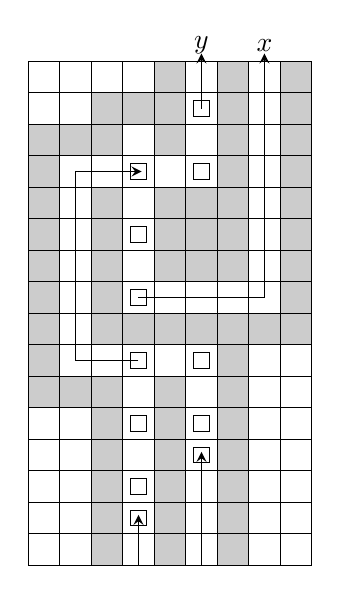
\begin{tikzpicture}[scale=0.40]
			
	%		\foreach \y in {1,...,16}
	%		\node at (0,\y) {\y};
			
	%		\foreach \x in {1,...,9}
	%		\node at (\x,0) {\x};
			
			\foreach \x in {0,...,9}
			\draw (\x+0.5,0.5)--(\x+0.5,16.5);
			
			\foreach \y in {0,...,16}
			\draw (0.5,\y+0.5)--(9.5,\y+0.5);
			
			
			\foreach \x in {4}
			\foreach \y in {2,3,5,7,9,11,13}
			\draw (\x-0.25,\y-0.25) -- (\x+0.25,\y-0.25) -- (\x+0.25,\y+0.25) -- (\x-0.25,\y+0.25) -- cycle;
			
			\foreach \x in {6}
			\foreach \y in {4,5,7,13,15}
			\draw (\x-0.25,\y-0.25) -- (\x+0.25,\y-0.25) -- (\x+0.25,\y+0.25) -- (\x-0.25,\y+0.25) -- cycle;
			
			\draw [semithick,->,>=stealth] (4,0.5) -- (4,2+0.1);
			\draw [semithick,->,>=stealth] (6,0.5) -- (6,4+0.1);
			
			\draw [semithick,->,>=stealth] (4,7) -- (2,7) -- (2,13) -- (4+0.1,13);
			
			\draw [semithick,->,>=stealth] (4,9) -- (8,9) -- (8,16+0.75);
			\draw [semithick,->,>=stealth] (6,15) -- (6,16+0.75);
			
			\node at (6,17) {$y$};
			\node at (8,17) {$x$};
			
			
			\foreach \x in {1}	
			\foreach \y in {6,...,14}
			\draw [fill = gray!40] (\x-0.5,\y-0.5) -- (\x+0.5,\y-0.5) -- (\x+0.5,\y+0.5) -- (\x-0.5,\y+0.5) -- cycle;	
			
			\foreach \x in {2}	
			\foreach \y in {6,14}
			\draw [fill = gray!40] (\x-0.5,\y-0.5) -- (\x+0.5,\y-0.5) -- (\x+0.5,\y+0.5) -- (\x-0.5,\y+0.5) -- cycle;	
			
			\foreach \x in {3}	
			\foreach \y in {1,...,6,8,9,10,11,12,14,15}
			\draw [fill = gray!40] (\x-0.5,\y-0.5) -- (\x+0.5,\y-0.5) -- (\x+0.5,\y+0.5) -- (\x-0.5,\y+0.5) -- cycle;	
			
			\foreach \x in {4}	
			\foreach \y in {8,15}
			\draw [fill = gray!40] (\x-0.5,\y-0.5) -- (\x+0.5,\y-0.5) -- (\x+0.5,\y+0.5) -- (\x-0.5,\y+0.5) -- cycle;	
			
			\foreach \x in {5}	
			\foreach \y in {1,...,6,8,10,11,12,14,15,16}
			\draw [fill = gray!40] (\x-0.5,\y-0.5) -- (\x+0.5,\y-0.5) -- (\x+0.5,\y+0.5) -- (\x-0.5,\y+0.5) -- cycle;	
			
			\foreach \x in {6}	
			\foreach \y in {8,10,11,12}
			\draw [fill = gray!40] (\x-0.5,\y-0.5) -- (\x+0.5,\y-0.5) -- (\x+0.5,\y+0.5) -- (\x-0.5,\y+0.5) -- cycle;	
			
			\foreach \x in {7}	
			\foreach \y in {1,...,8,10,11,12,13,14,15,16}
			\draw [fill = gray!40] (\x-0.5,\y-0.5) -- (\x+0.5,\y-0.5) -- (\x+0.5,\y+0.5) -- (\x-0.5,\y+0.5) -- cycle;	
			
			\foreach \x in {8}	
			\foreach \y in {8}
			\draw [fill = gray!40] (\x-0.5,\y-0.5) -- (\x+0.5,\y-0.5) -- (\x+0.5,\y+0.5) -- (\x-0.5,\y+0.5) -- cycle;	
			
			\foreach \x in {9}	
			\foreach \y in {8,...,16}
			\draw [fill = gray!40] (\x-0.5,\y-0.5) -- (\x+0.5,\y-0.5) -- (\x+0.5,\y+0.5) -- (\x-0.5,\y+0.5) -- cycle;	
			
		\end{tikzpicture}
		\caption {Crossover gadget}
		\label {Fig_crossover_gadget}
	\end{figure}
	
	
	\begin{figure}[h]
		\centering
		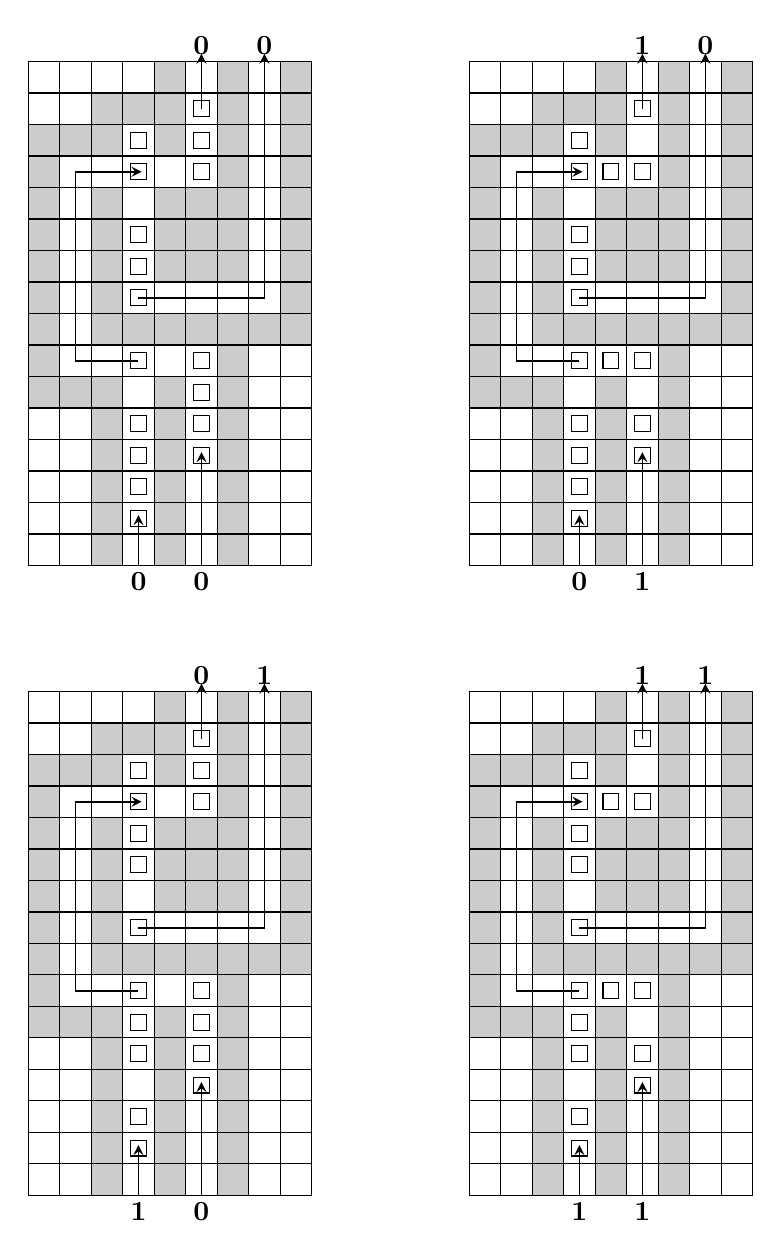
\begin{tikzpicture}[scale=0.40]
			
	%		\foreach \y in {1,...,16}
	%		\node at (0,\y) {\y};
			
			\foreach \x in {0,...,9}
			\draw (\x+0.5,0.5)--(\x+0.5,16.5);
			
			\foreach \y in {0,...,16}
			\draw (0.5,\y+0.5)--(9.5,\y+0.5);
			
			\node at (4,0) {\bf{0}};
			\node at (6,0) {\bf{0}};
			
			\node at (6,17) {\bf{0}};
			\node at (8,17) {\bf{0}};
			
			
			\foreach \x in {4}
			\foreach \y in {2,3,4,5,7,9,10,11,13,14}
			\draw (\x-0.25,\y-0.25) -- (\x+0.25,\y-0.25) -- (\x+0.25,\y+0.25) -- (\x-0.25,\y+0.25) -- cycle;
			
			\foreach \x in {6}
			\foreach \y in {4,5,6,7,13,14,15}
			\draw (\x-0.25,\y-0.25) -- (\x+0.25,\y-0.25) -- (\x+0.25,\y+0.25) -- (\x-0.25,\y+0.25) -- cycle;
			
			\draw [semithick,->,>=stealth] (4,0.5) -- (4,2+0.1);
			\draw [semithick,->,>=stealth] (6,0.5) -- (6,4+0.1);
			
			\draw [semithick,->,>=stealth] (4,7) -- (2,7) -- (2,13) -- (4+0.1,13);
			
			\draw [semithick,->,>=stealth] (4,9) -- (8,9) -- (8,16+0.75);
			\draw [semithick,->,>=stealth] (6,15) -- (6,16+0.75);
			
			
			\foreach \x in {1}	
			\foreach \y in {6,...,14}
			\draw [fill = gray!40] (\x-0.5,\y-0.5) -- (\x+0.5,\y-0.5) -- (\x+0.5,\y+0.5) -- (\x-0.5,\y+0.5) -- cycle;	
			
			\foreach \x in {2}	
			\foreach \y in {6,14}
			\draw [fill = gray!40] (\x-0.5,\y-0.5) -- (\x+0.5,\y-0.5) -- (\x+0.5,\y+0.5) -- (\x-0.5,\y+0.5) -- cycle;	
			
			\foreach \x in {3}	
			\foreach \y in {1,...,6,8,9,10,11,12,14,15}
			\draw [fill = gray!40] (\x-0.5,\y-0.5) -- (\x+0.5,\y-0.5) -- (\x+0.5,\y+0.5) -- (\x-0.5,\y+0.5) -- cycle;	
			
			\foreach \x in {4}	
			\foreach \y in {8,15}
			\draw [fill = gray!40] (\x-0.5,\y-0.5) -- (\x+0.5,\y-0.5) -- (\x+0.5,\y+0.5) -- (\x-0.5,\y+0.5) -- cycle;	
			
			\foreach \x in {5}	
			\foreach \y in {1,...,6,8,10,11,12,14,15,16}
			\draw [fill = gray!40] (\x-0.5,\y-0.5) -- (\x+0.5,\y-0.5) -- (\x+0.5,\y+0.5) -- (\x-0.5,\y+0.5) -- cycle;	
			
			\foreach \x in {6}	
			\foreach \y in {8,10,11,12}
			\draw [fill = gray!40] (\x-0.5,\y-0.5) -- (\x+0.5,\y-0.5) -- (\x+0.5,\y+0.5) -- (\x-0.5,\y+0.5) -- cycle;	
			
			\foreach \x in {7}	
			\foreach \y in {1,...,8,10,11,12,13,14,15,16}
			\draw [fill = gray!40] (\x-0.5,\y-0.5) -- (\x+0.5,\y-0.5) -- (\x+0.5,\y+0.5) -- (\x-0.5,\y+0.5) -- cycle;	
			
			\foreach \x in {8}	
			\foreach \y in {8}
			\draw [fill = gray!40] (\x-0.5,\y-0.5) -- (\x+0.5,\y-0.5) -- (\x+0.5,\y+0.5) -- (\x-0.5,\y+0.5) -- cycle;	
			
			\foreach \x in {9}	
			\foreach \y in {8,...,16}
			\draw [fill = gray!40] (\x-0.5,\y-0.5) -- (\x+0.5,\y-0.5) -- (\x+0.5,\y+0.5) -- (\x-0.5,\y+0.5) -- cycle;	
			
			
			\begin{scope}[xshift=14cm]
		%		\foreach \y in {1,...,16}
		%		\node at (0,\y) {\y};
				
				\foreach \x in {0,...,9}
				\draw (\x+0.5,0.5)--(\x+0.5,16.5);
				
				\foreach \y in {0,...,16}
				\draw (0.5,\y+0.5)--(9.5,\y+0.5);
				
				\node at (4,0) {\bf{0}};
				\node at (6,0) {\bf{1}};
				
				\node at (6,17) {\bf{1}};
				\node at (8,17) {\bf{0}};
				
				
				\foreach \x in {4}
				\foreach \y in {2,3,4,5,7,9,10,11,13,14}
				\draw (\x-0.25,\y-0.25) -- (\x+0.25,\y-0.25) -- (\x+0.25,\y+0.25) -- (\x-0.25,\y+0.25) -- cycle;
				
				\foreach \x in {5}
				\foreach \y in {7,13}
				\draw (\x-0.25,\y-0.25) -- (\x+0.25,\y-0.25) -- (\x+0.25,\y+0.25) -- (\x-0.25,\y+0.25) -- cycle;
				
				\foreach \x in {6}
				\foreach \y in {4,5,7,13,15}
				\draw (\x-0.25,\y-0.25) -- (\x+0.25,\y-0.25) -- (\x+0.25,\y+0.25) -- (\x-0.25,\y+0.25) -- cycle;
				
				\draw [semithick,->,>=stealth] (4,0.5) -- (4,2+0.1);
				\draw [semithick,->,>=stealth] (6,0.5) -- (6,4+0.1);
				
				\draw [semithick,->,>=stealth] (4,7) -- (2,7) -- (2,13) -- (4+0.1,13);
				
				\draw [semithick,->,>=stealth] (4,9) -- (8,9) -- (8,16+0.75);
				\draw [semithick,->,>=stealth] (6,15) -- (6,16+0.75);
				
				
				\foreach \x in {1}	
				\foreach \y in {6,...,14}
				\draw [fill = gray!40] (\x-0.5,\y-0.5) -- (\x+0.5,\y-0.5) -- (\x+0.5,\y+0.5) -- (\x-0.5,\y+0.5) -- cycle;	
				
				\foreach \x in {2}	
				\foreach \y in {6,14}
				\draw [fill = gray!40] (\x-0.5,\y-0.5) -- (\x+0.5,\y-0.5) -- (\x+0.5,\y+0.5) -- (\x-0.5,\y+0.5) -- cycle;	
				
				\foreach \x in {3}	
				\foreach \y in {1,...,6,8,9,10,11,12,14,15}
				\draw [fill = gray!40] (\x-0.5,\y-0.5) -- (\x+0.5,\y-0.5) -- (\x+0.5,\y+0.5) -- (\x-0.5,\y+0.5) -- cycle;	
				
				\foreach \x in {4}	
				\foreach \y in {8,15}
				\draw [fill = gray!40] (\x-0.5,\y-0.5) -- (\x+0.5,\y-0.5) -- (\x+0.5,\y+0.5) -- (\x-0.5,\y+0.5) -- cycle;	
				
				\foreach \x in {5}	
				\foreach \y in {1,...,6,8,10,11,12,14,15,16}
				\draw [fill = gray!40] (\x-0.5,\y-0.5) -- (\x+0.5,\y-0.5) -- (\x+0.5,\y+0.5) -- (\x-0.5,\y+0.5) -- cycle;	
				
				\foreach \x in {6}	
				\foreach \y in {8,10,11,12}
				\draw [fill = gray!40] (\x-0.5,\y-0.5) -- (\x+0.5,\y-0.5) -- (\x+0.5,\y+0.5) -- (\x-0.5,\y+0.5) -- cycle;	
				
				\foreach \x in {7}	
				\foreach \y in {1,...,8,10,11,12,13,14,15,16}
				\draw [fill = gray!40] (\x-0.5,\y-0.5) -- (\x+0.5,\y-0.5) -- (\x+0.5,\y+0.5) -- (\x-0.5,\y+0.5) -- cycle;	
				
				\foreach \x in {8}	
				\foreach \y in {8}
				\draw [fill = gray!40] (\x-0.5,\y-0.5) -- (\x+0.5,\y-0.5) -- (\x+0.5,\y+0.5) -- (\x-0.5,\y+0.5) -- cycle;	
				
				\foreach \x in {9}	
				\foreach \y in {8,...,16}
				\draw [fill = gray!40] (\x-0.5,\y-0.5) -- (\x+0.5,\y-0.5) -- (\x+0.5,\y+0.5) -- (\x-0.5,\y+0.5) -- cycle;	
			\end{scope}
			
			
			\begin{scope}[yshift=-20cm]
		%		\foreach \y in {1,...,16}
		%		\node at (0,\y) {\y};
				
				\foreach \x in {0,...,9}
				\draw (\x+0.5,0.5)--(\x+0.5,16.5);
				
				\foreach \y in {0,...,16}
				\draw (0.5,\y+0.5)--(9.5,\y+0.5);
				
				\node at (4,0) {\bf{1}};
				\node at (6,0) {\bf{0}};
				
				\node at (6,17) {\bf{0}};
				\node at (8,17) {\bf{1}};
				
				
				\foreach \x in {4}
				\foreach \y in {2,3,5,6,7,9,11,12,13,14}
				\draw (\x-0.25,\y-0.25) -- (\x+0.25,\y-0.25) -- (\x+0.25,\y+0.25) -- (\x-0.25,\y+0.25) -- cycle;
				
				\foreach \x in {6}
				\foreach \y in {4,5,6,7,13,14,15}
				\draw (\x-0.25,\y-0.25) -- (\x+0.25,\y-0.25) -- (\x+0.25,\y+0.25) -- (\x-0.25,\y+0.25) -- cycle;
				
				\draw [semithick,->,>=stealth] (4,0.5) -- (4,2+0.1);
				\draw [semithick,->,>=stealth] (6,0.5) -- (6,4+0.1);
				
				\draw [semithick,->,>=stealth] (4,7) -- (2,7) -- (2,13) -- (4+0.1,13);
				
				\draw [semithick,->,>=stealth] (4,9) -- (8,9) -- (8,16+0.75);
				\draw [semithick,->,>=stealth] (6,15) -- (6,16+0.75);
				
				
				\foreach \x in {1}	
				\foreach \y in {6,...,14}
				\draw [fill = gray!40] (\x-0.5,\y-0.5) -- (\x+0.5,\y-0.5) -- (\x+0.5,\y+0.5) -- (\x-0.5,\y+0.5) -- cycle;	
				
				\foreach \x in {2}	
				\foreach \y in {6,14}
				\draw [fill = gray!40] (\x-0.5,\y-0.5) -- (\x+0.5,\y-0.5) -- (\x+0.5,\y+0.5) -- (\x-0.5,\y+0.5) -- cycle;	
				
				\foreach \x in {3}	
				\foreach \y in {1,...,6,8,9,10,11,12,14,15}
				\draw [fill = gray!40] (\x-0.5,\y-0.5) -- (\x+0.5,\y-0.5) -- (\x+0.5,\y+0.5) -- (\x-0.5,\y+0.5) -- cycle;	
				
				\foreach \x in {4}	
				\foreach \y in {8,15}
				\draw [fill = gray!40] (\x-0.5,\y-0.5) -- (\x+0.5,\y-0.5) -- (\x+0.5,\y+0.5) -- (\x-0.5,\y+0.5) -- cycle;	
				
				\foreach \x in {5}	
				\foreach \y in {1,...,6,8,10,11,12,14,15,16}
				\draw [fill = gray!40] (\x-0.5,\y-0.5) -- (\x+0.5,\y-0.5) -- (\x+0.5,\y+0.5) -- (\x-0.5,\y+0.5) -- cycle;	
				
				\foreach \x in {6}	
				\foreach \y in {8,10,11,12}
				\draw [fill = gray!40] (\x-0.5,\y-0.5) -- (\x+0.5,\y-0.5) -- (\x+0.5,\y+0.5) -- (\x-0.5,\y+0.5) -- cycle;	
				
				\foreach \x in {7}	
				\foreach \y in {1,...,8,10,11,12,13,14,15,16}
				\draw [fill = gray!40] (\x-0.5,\y-0.5) -- (\x+0.5,\y-0.5) -- (\x+0.5,\y+0.5) -- (\x-0.5,\y+0.5) -- cycle;	
				
				\foreach \x in {8}	
				\foreach \y in {8}
				\draw [fill = gray!40] (\x-0.5,\y-0.5) -- (\x+0.5,\y-0.5) -- (\x+0.5,\y+0.5) -- (\x-0.5,\y+0.5) -- cycle;	
				
				\foreach \x in {9}	
				\foreach \y in {8,...,16}
				\draw [fill = gray!40] (\x-0.5,\y-0.5) -- (\x+0.5,\y-0.5) -- (\x+0.5,\y+0.5) -- (\x-0.5,\y+0.5) -- cycle;	
			\end{scope}
			
			
			\begin{scope}[xshift=14cm,yshift=-20cm]
		%		\foreach \y in {1,...,16}
		%		\node at (0,\y) {\y};
				
				\foreach \x in {0,...,9}
				\draw (\x+0.5,0.5)--(\x+0.5,16.5);
				
				\foreach \y in {0,...,16}
				\draw (0.5,\y+0.5)--(9.5,\y+0.5);
				
				\node at (4,0) {\bf{1}};
				\node at (6,0) {\bf{1}};
				
				\node at (6,17) {\bf{1}};
				\node at (8,17) {\bf{1}};
				
				
				\foreach \x in {4}
				\foreach \y in {2,3,5,6,7,9,11,12,13,14}
				\draw (\x-0.25,\y-0.25) -- (\x+0.25,\y-0.25) -- (\x+0.25,\y+0.25) -- (\x-0.25,\y+0.25) -- cycle;
				
				\foreach \x in {5}
				\foreach \y in {7,13}
				\draw (\x-0.25,\y-0.25) -- (\x+0.25,\y-0.25) -- (\x+0.25,\y+0.25) -- (\x-0.25,\y+0.25) -- cycle;
				
				\foreach \x in {6}
				\foreach \y in {4,5,7,13,15}
				\draw (\x-0.25,\y-0.25) -- (\x+0.25,\y-0.25) -- (\x+0.25,\y+0.25) -- (\x-0.25,\y+0.25) -- cycle;
				
				\draw [semithick,->,>=stealth] (4,0.5) -- (4,2+0.1);
				\draw [semithick,->,>=stealth] (6,0.5) -- (6,4+0.1);
				
				\draw [semithick,->,>=stealth] (4,7) -- (2,7) -- (2,13) -- (4+0.1,13);
				
				\draw [semithick,->,>=stealth] (4,9) -- (8,9) -- (8,16+0.75);
				\draw [semithick,->,>=stealth] (6,15) -- (6,16+0.75);
				
				
				\foreach \x in {1}	
				\foreach \y in {6,...,14}
				\draw [fill = gray!40] (\x-0.5,\y-0.5) -- (\x+0.5,\y-0.5) -- (\x+0.5,\y+0.5) -- (\x-0.5,\y+0.5) -- cycle;	
				
				\foreach \x in {2}	
				\foreach \y in {6,14}
				\draw [fill = gray!40] (\x-0.5,\y-0.5) -- (\x+0.5,\y-0.5) -- (\x+0.5,\y+0.5) -- (\x-0.5,\y+0.5) -- cycle;	
				
				\foreach \x in {3}	
				\foreach \y in {1,...,6,8,9,10,11,12,14,15}
				\draw [fill = gray!40] (\x-0.5,\y-0.5) -- (\x+0.5,\y-0.5) -- (\x+0.5,\y+0.5) -- (\x-0.5,\y+0.5) -- cycle;	
				
				\foreach \x in {4}	
				\foreach \y in {8,15}
				\draw [fill = gray!40] (\x-0.5,\y-0.5) -- (\x+0.5,\y-0.5) -- (\x+0.5,\y+0.5) -- (\x-0.5,\y+0.5) -- cycle;	
				
				\foreach \x in {5}	
				\foreach \y in {1,...,6,8,10,11,12,14,15,16}
				\draw [fill = gray!40] (\x-0.5,\y-0.5) -- (\x+0.5,\y-0.5) -- (\x+0.5,\y+0.5) -- (\x-0.5,\y+0.5) -- cycle;	
				
				\foreach \x in {6}	
				\foreach \y in {8,10,11,12}
				\draw [fill = gray!40] (\x-0.5,\y-0.5) -- (\x+0.5,\y-0.5) -- (\x+0.5,\y+0.5) -- (\x-0.5,\y+0.5) -- cycle;	
				
				\foreach \x in {7}	
				\foreach \y in {1,...,8,10,11,12,13,14,15,16}
				\draw [fill = gray!40] (\x-0.5,\y-0.5) -- (\x+0.5,\y-0.5) -- (\x+0.5,\y+0.5) -- (\x-0.5,\y+0.5) -- cycle;	
				
				\foreach \x in {8}	
				\foreach \y in {8}
				\draw [fill = gray!40] (\x-0.5,\y-0.5) -- (\x+0.5,\y-0.5) -- (\x+0.5,\y+0.5) -- (\x-0.5,\y+0.5) -- cycle;	
				
				\foreach \x in {9}	
				\foreach \y in {8,...,16}
				\draw [fill = gray!40] (\x-0.5,\y-0.5) -- (\x+0.5,\y-0.5) -- (\x+0.5,\y+0.5) -- (\x-0.5,\y+0.5) -- cycle;	
			\end{scope}
			
		\end{tikzpicture}
		\caption {Four cases of solving a crossover gadget}
		\label {Fig_crossover_gadget_cases}
	\end{figure}
	
	
	\subsubsection{Complexity of reduction and board size.}
	
	Let's consider an instance of the \textsc{3-SAT} problem that consists of a collection of clauses $C = \{C_1,\ldots,C_m\}$ over Boolean variables $X=\{x_1,\ldots,x_n\}$. 
	
	Let us represent a Boolean formula as a bipartite incidence graph with $n$ variables in one part and $m$ clauses in the other, where the edge $(x,C)$ indicates that the variable $x$ participates in clause $C$. We obtain a bipartite graph on $n+m$ vertices and $3m$ edges, based on which we construct an \textsc{Evolomino} board. An example of an incidence graph of a Boolean formula is shown in Fig.~\ref{Fig_full_board} with solid edges corresponding to non-inverted variables and dashed edges to inverted variables.
	
	Let's estimate the total number of gadgets required:
	\begin{itemize}
		\item $n$ variable and wire gadgets, one for each Boolean variable $x_1,\ldots,x_n$; 
		\item $m$ clause gadgets, one for each clause $C_1,\ldots,C_m$;
		\item $3m - n$ split gadgets, to assign a wire to each edge;
		\item at most $3m$ negation gadgets, one for each edge for an inverted variable;
		\item at most $\binom{3m}{2}$ crossover gadgets, one for each crossing of edges.
	\end{itemize}
	
	Regarding the crossing number, we note that the graph can always be drawn so that no three edges are crossing at a single point. If the edges are drawn as straight lines, then in the worst case no more than any two edges can cross. More precise estimates of the crossing number of a bipartite graph can be obtained from graph theory, see, for example, Turán's brick factory problem~\cite{Székely2016,Zarankiewicz1955}.
	
	Given that each gadget, except the wire, has a constant size, we get that an instance of the \textsc{3-SAT} problem on $m$ clauses and $n$ variables reduces to an \textsc{Evolomino} puzzle on a board of size $O(m^2+n) \times O(m^2+n)$. 
	As for the wires, they only need to carry the signal from the variable gadgets to the clause gadgets, so their size is proportional to the size of the rest of the board.
	Therefore, the reduction is performed in polynomial time.
	
	Note that the board size and the complexity of the reduction can be significantly reduced if we exclude the crossover gadgets and consider the reduction from the NP-complete \textsc{planar 3-SAT} problem~\cite{Lichtenstein1982} where the incidence graph of a Boolean formula can be embedded on a plane. However, we decided that if the crossover is possible, it would be correct to consider a more general construction.
	
	
	\subsubsection{An example of constructing the entire puzzle board.}
	
	An example of constructing the \textsc{Evolomino} board for the \textsc{3-SAT} instance $C_1 \wedge C_2$, where $C_1 = (x_1 \vee \bar{x}_2 \vee x_3)$ and $C_2 = (x_2 \vee \bar{x}_3 \vee \bar{x}_4)$ is depicted in Fig.~\ref{Fig_full_board}. 
	
	The board size is $42 \times 21$ and includes:
	\begin{itemize}
		\item 4 variable and wire gadgets for $x_1$, $x_2$, $x_3$, and $x_4$;
		\item 2 clause gadgets for $C_1$ and $C_2$;
		\item 2 split gadgets for $x_2$ and $x_3$;
		\item 3 negation gadgets for $(x_2,C_1)$, $(x_3,C_2)$, and $(x_4,C_2)$;
		\item 1 crossover gadget for $(x_2,C_2)$ and $(x_3,C_1)$.
	\end{itemize}
	
	An example of a puzzle solution that satisfies all the clauses and corresponds to the truth assignment $x_1 = 0$, $x_2 = 1$, $x_3 = 1$, $x_4 = 0$ is shown in Fig.~\ref{Fig_full_board_solution}.
	
	\begin{figure}[t]
		\centering
		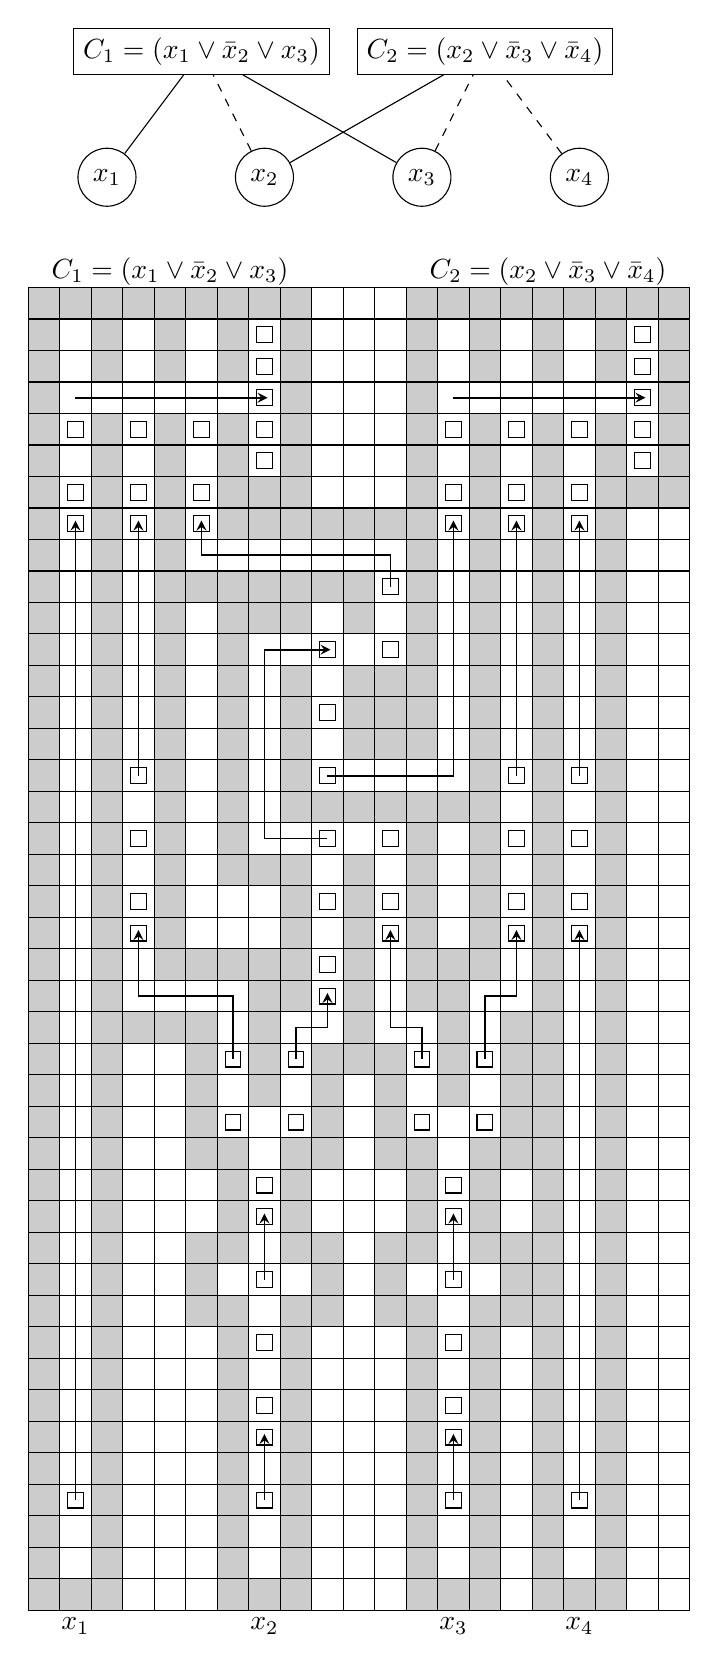
\begin{tikzpicture}[scale=0.40]
			
		%	\foreach \x in {1,...,21}
		%	{
		%		\node at (\x,0) {\x};
		%		\node at (\x,43) {\x};
		%	}
			
		%	\foreach \y in {1,...,42}
		%	{
		%		\node at (0,\y) {\y};
		%		\node at (22,\y) {\y};
		%	}
			
			\foreach \x in {0,...,21}
			\draw (\x+0.5,0.5)--(\x+0.5,42.5);
			
			\foreach \x in {0,...,42}
			\draw (0.5,\x+0.5)--(21.5,\x+0.5);
			
			
			\foreach \x in {1}	
			\foreach \y in {1,...,42}
			\draw [fill = gray!40] (\x-0.5,\y-0.5) -- (\x+0.5,\y-0.5) -- (\x+0.5,\y+0.5) -- (\x-0.5,\y+0.5) -- cycle;	
			
			\foreach \x in {2}	
			\foreach \y in {1,42}
			\draw [fill = gray!40] (\x-0.5,\y-0.5) -- (\x+0.5,\y-0.5) -- (\x+0.5,\y+0.5) -- (\x-0.5,\y+0.5) -- cycle;	
			
			\foreach \x in {3}	
			\foreach \y in {1,...,38,40,41,42}
			\draw [fill = gray!40] (\x-0.5,\y-0.5) -- (\x+0.5,\y-0.5) -- (\x+0.5,\y+0.5) -- (\x-0.5,\y+0.5) -- cycle;	
			
			\foreach \x in {4}	
			\foreach \y in {19,42}
			\draw [fill = gray!40] (\x-0.5,\y-0.5) -- (\x+0.5,\y-0.5) -- (\x+0.5,\y+0.5) -- (\x-0.5,\y+0.5) -- cycle;	
			
			\foreach \x in {5}	
			\foreach \y in {19,21,22,...,38,40,41,42}
			\draw [fill = gray!40] (\x-0.5,\y-0.5) -- (\x+0.5,\y-0.5) -- (\x+0.5,\y+0.5) -- (\x-0.5,\y+0.5) -- cycle;	
			
			\foreach \x in {6}	
			\foreach \y in {10,11,12,15,16,17,18,19,21,33,42}
			\draw [fill = gray!40] (\x-0.5,\y-0.5) -- (\x+0.5,\y-0.5) -- (\x+0.5,\y+0.5) -- (\x-0.5,\y+0.5) -- cycle;	
			
			\foreach \x in {7}	
			\foreach \y in {1,...,10,12,13,14,15,21,24,25,...,33,35,36,37,38,40,41,42}
			\draw [fill = gray!40] (\x-0.5,\y-0.5) -- (\x+0.5,\y-0.5) -- (\x+0.5,\y+0.5) -- (\x-0.5,\y+0.5) -- cycle;	
			
			\foreach \x in {8}	
			\foreach \y in {1,17,18,...,21,24,32,33,35,36,42}
			\draw [fill = gray!40] (\x-0.5,\y-0.5) -- (\x+0.5,\y-0.5) -- (\x+0.5,\y+0.5) -- (\x-0.5,\y+0.5) -- cycle;	
			
			\foreach \x in {9}	
			\foreach \y in {1,...,10,12,13,14,15,20,21,22,23,24,26,27,28,29,30,32,33,35,36,...,42}
			\draw [fill = gray!40] (\x-0.5,\y-0.5) -- (\x+0.5,\y-0.5) -- (\x+0.5,\y+0.5) -- (\x-0.5,\y+0.5) -- cycle;	
			
			\foreach \x in {10}	
			\foreach \y in {10,11,12,15,16,17,18,26,33,35}
			\draw [fill = gray!40] (\x-0.5,\y-0.5) -- (\x+0.5,\y-0.5) -- (\x+0.5,\y+0.5) -- (\x-0.5,\y+0.5) -- cycle;	
			
			\foreach \x in {11}	
			\foreach \y in {18,...,24,26,28,29,30,32,33,35}
			\draw [fill = gray!40] (\x-0.5,\y-0.5) -- (\x+0.5,\y-0.5) -- (\x+0.5,\y+0.5) -- (\x-0.5,\y+0.5) -- cycle;	
			
			\foreach \x in {12}	
			\foreach \y in {10,11,12,15,16,17,18,26,28,29,30,35}
			\draw [fill = gray!40] (\x-0.5,\y-0.5) -- (\x+0.5,\y-0.5) -- (\x+0.5,\y+0.5) -- (\x-0.5,\y+0.5) -- cycle;	
			
			\foreach \x in {13}	
			\foreach \y in {1,...,10,12,13,14,15,20,21,...,26,28,29,...,42}
			\draw [fill = gray!40] (\x-0.5,\y-0.5) -- (\x+0.5,\y-0.5) -- (\x+0.5,\y+0.5) -- (\x-0.5,\y+0.5) -- cycle;	
			
			\foreach \x in {14}	
			\foreach \y in {1,17,18,...,21,26,42}
			\draw [fill = gray!40] (\x-0.5,\y-0.5) -- (\x+0.5,\y-0.5) -- (\x+0.5,\y+0.5) -- (\x-0.5,\y+0.5) -- cycle;	
			
			\foreach \x in {15}	
			\foreach \y in {1,...,10,12,13,14,15,21,22,...,38,40,41,42}
			\draw [fill = gray!40] (\x-0.5,\y-0.5) -- (\x+0.5,\y-0.5) -- (\x+0.5,\y+0.5) -- (\x-0.5,\y+0.5) -- cycle;	
			
			\foreach \x in {16}	
			\foreach \y in {10,11,12,15,16,...,19,42}
			\draw [fill = gray!40] (\x-0.5,\y-0.5) -- (\x+0.5,\y-0.5) -- (\x+0.5,\y+0.5) -- (\x-0.5,\y+0.5) -- cycle;	
			
			\foreach \x in {17}	
			\foreach \y in {1,...,38,40,41,42}
			\draw [fill = gray!40] (\x-0.5,\y-0.5) -- (\x+0.5,\y-0.5) -- (\x+0.5,\y+0.5) -- (\x-0.5,\y+0.5) -- cycle;	
			
			\foreach \x in {18}	
			\foreach \y in {1,42}
			\draw [fill = gray!40] (\x-0.5,\y-0.5) -- (\x+0.5,\y-0.5) -- (\x+0.5,\y+0.5) -- (\x-0.5,\y+0.5) -- cycle;	
			
			\foreach \x in {19}	
			\foreach \y in {1,...,38,40,41,42}
			\draw [fill = gray!40] (\x-0.5,\y-0.5) -- (\x+0.5,\y-0.5) -- (\x+0.5,\y+0.5) -- (\x-0.5,\y+0.5) -- cycle;	
			
			\foreach \x in {20}	
			\foreach \y in {36,42}
			\draw [fill = gray!40] (\x-0.5,\y-0.5) -- (\x+0.5,\y-0.5) -- (\x+0.5,\y+0.5) -- (\x-0.5,\y+0.5) -- cycle;	
			
			\foreach \x in {21}	
			\foreach \y in {36,...,42}
			\draw [fill = gray!40] (\x-0.5,\y-0.5) -- (\x+0.5,\y-0.5) -- (\x+0.5,\y+0.5) -- (\x-0.5,\y+0.5) -- cycle;	
			
			
			
			
			\foreach \x in {2}
			\foreach \y in {4,35,36,38}
			\draw (\x-0.25,\y-0.25) -- (\x+0.25,\y-0.25) -- (\x+0.25,\y+0.25) -- (\x-0.25,\y+0.25) -- cycle;
			
			\foreach \x in {4}
			\foreach \y in {22,23,25,27,35,36,38}
			\draw (\x-0.25,\y-0.25) -- (\x+0.25,\y-0.25) -- (\x+0.25,\y+0.25) -- (\x-0.25,\y+0.25) -- cycle;
			
			\foreach \x in {6}
			\foreach \y in {35,36,38}
			\draw (\x-0.25,\y-0.25) -- (\x+0.25,\y-0.25) -- (\x+0.25,\y+0.25) -- (\x-0.25,\y+0.25) -- cycle;
			
			\foreach \x in {7}
			\foreach \y in {16,18}
			\draw (\x-0.25,\y-0.25) -- (\x+0.25,\y-0.25) -- (\x+0.25,\y+0.25) -- (\x-0.25,\y+0.25) -- cycle;
			
			\foreach \x in {8}
			\foreach \y in {4,6,7,9,11,13,14,37,38,39,40,41}
			\draw (\x-0.25,\y-0.25) -- (\x+0.25,\y-0.25) -- (\x+0.25,\y+0.25) -- (\x-0.25,\y+0.25) -- cycle;
			
			\foreach \x in {9}
			\foreach \y in {16,18}
			\draw (\x-0.25,\y-0.25) -- (\x+0.25,\y-0.25) -- (\x+0.25,\y+0.25) -- (\x-0.25,\y+0.25) -- cycle;
			
			\foreach \x in {10}
			\foreach \y in {20,21,23,25,27,29,31}
			\draw (\x-0.25,\y-0.25) -- (\x+0.25,\y-0.25) -- (\x+0.25,\y+0.25) -- (\x-0.25,\y+0.25) -- cycle;
			
			\foreach \x in {12}
			\foreach \y in {22,23,25,31,33}
			\draw (\x-0.25,\y-0.25) -- (\x+0.25,\y-0.25) -- (\x+0.25,\y+0.25) -- (\x-0.25,\y+0.25) -- cycle;
			
			\foreach \x in {13}
			\foreach \y in {16,18}
			\draw (\x-0.25,\y-0.25) -- (\x+0.25,\y-0.25) -- (\x+0.25,\y+0.25) -- (\x-0.25,\y+0.25) -- cycle;
			
			\foreach \x in {14}
			\foreach \y in {4,6,7,9,11,13,14,35,36,38}
			\draw (\x-0.25,\y-0.25) -- (\x+0.25,\y-0.25) -- (\x+0.25,\y+0.25) -- (\x-0.25,\y+0.25) -- cycle;
			
			\foreach \x in {15}
			\foreach \y in {16,18}
			\draw (\x-0.25,\y-0.25) -- (\x+0.25,\y-0.25) -- (\x+0.25,\y+0.25) -- (\x-0.25,\y+0.25) -- cycle;
			
			\foreach \x in {16}
			\foreach \y in {22,23,25,27,35,36,38}
			\draw (\x-0.25,\y-0.25) -- (\x+0.25,\y-0.25) -- (\x+0.25,\y+0.25) -- (\x-0.25,\y+0.25) -- cycle;
			
			\foreach \x in {18}
			\foreach \y in {4,22,23,25,27,35,36,38}
			\draw (\x-0.25,\y-0.25) -- (\x+0.25,\y-0.25) -- (\x+0.25,\y+0.25) -- (\x-0.25,\y+0.25) -- cycle;
			
			\foreach \x in {20}
			\foreach \y in {37,38,39,40,41}
			\draw (\x-0.25,\y-0.25) -- (\x+0.25,\y-0.25) -- (\x+0.25,\y+0.25) -- (\x-0.25,\y+0.25) -- cycle;
			
			
			
			\foreach \x in {8,14}
			{
				\draw [semithick,->,>=stealth] (\x,4) -- (\x,6+0.1);
				\draw [semithick,->,>=stealth] (\x,11) -- (\x,13+0.1);			
			}
			
		
			\draw [semithick,->,>=stealth] (10,25) -- (8,25) -- (8,31) -- (10+0.1,31);
			
			\draw [semithick,->,>=stealth] (9,18) -- (9,19) -- (10,19) -- (10,20+0.1);
			\draw [semithick,->,>=stealth] (13,18) -- (13,19) -- (12,19) -- (12,22+0.1);
			
			\draw [semithick,->,>=stealth] (12,33) -- (12,34) -- (6,34) -- (6,35+0.1);
			
			\draw [semithick,->,>=stealth] (10,27) -- (14,27) -- (14,35+0.1);
			
			\draw [semithick,->,>=stealth] (7,18) -- (7,20) -- (4,20) -- (4,22+0.1);
			\draw [semithick,->,>=stealth] (15,18) -- (15,20) -- (16,20) -- (16,22+0.1);
			
			\foreach \x in {4,16,18}
			\draw [semithick,->,>=stealth] (\x,27) -- (\x,35+0.1);
			
			\draw [semithick,->,>=stealth] (2,4) -- (2,35+0.1);
			\draw [semithick,->,>=stealth] (18,4) -- (18,22+0.1);
			
			
			\draw [semithick,->,>=stealth] (2,39) -- (8+0.1,39);
			\draw [semithick,->,>=stealth] (14,39) -- (20+0.1,39);
			
			
			\node at (2,0) {$x_1$};
			\node at (8,0) {$x_2$};
			\node at (14,0) {$x_3$};
			\node at (18,0) {$x_4$};
			
			\node at (5,43) {$C_1=(x_1 \vee \bar{x}_2 \vee x_3)$};
			\node at (17,43) {$C_2=(x_2 \vee \bar{x}_3 \vee \bar{x}_4)$};
			
			
			
			\node (C1) [draw,rectangle] at (6,50) {$C_1=(x_1 \vee \bar{x}_2 \vee x_3)$};
			\node (C2) [draw,rectangle] at (15,50) {$C_2=(x_2 \vee \bar{x}_3 \vee \bar{x}_4)$};
			
			\node (x1) [draw,circle] at (3,46) {$x_1$};
			\node (x2) [draw,circle] at (8,46) {$x_2$};
			\node (x3) [draw,circle] at (13,46) {$x_3$};
			\node (x4) [draw,circle] at (18,46) {$x_4$};
			
			\draw (x1) -- (C1);
			\draw [dashed] (x2) -- (C1);
			\draw (x3) -- (C1);
			\draw (x2) -- (C2);
			\draw [dashed] (x3) -- (C2);
			\draw [dashed] (x4) -- (C2);
		
		\end{tikzpicture}
		\caption {An example of constructing a puzzle for the formula $(x_1 \vee \bar{x}_2 \vee x_3) \wedge (x_2 \vee \bar{x}_3 \vee \bar{x}_4)$}
		\label {Fig_full_board}
	\end{figure}
	
	
	
	
	\begin{figure}[t]
		\centering
		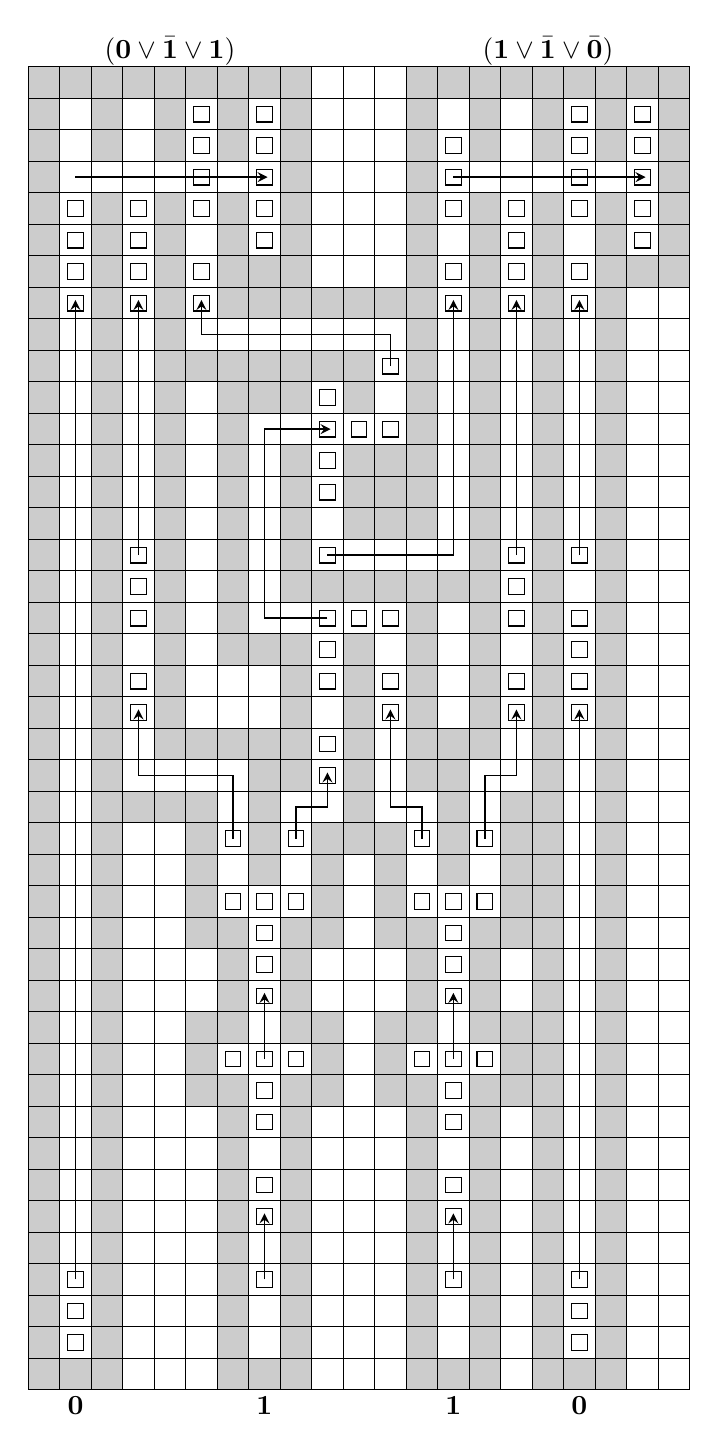
\begin{tikzpicture}[scale=0.40]
				
		%	\foreach \x in {1,...,21}
		%	{
		%		\node at (\x,0) {\x};
		%		\node at (\x,43) {\x};
		%	}
			
		%	\foreach \y in {1,...,42}
		%	{
		%		\node at (0,\y) {\y};
		%		\node at (22,\y) {\y};
		%	}
			
			\foreach \x in {0,...,21}
			\draw (\x+0.5,0.5)--(\x+0.5,42.5);
			
			\foreach \x in {0,...,42}
			\draw (0.5,\x+0.5)--(21.5,\x+0.5);
			
			
			\foreach \x in {1}	
			\foreach \y in {1,...,42}
			\draw [fill = gray!40] (\x-0.5,\y-0.5) -- (\x+0.5,\y-0.5) -- (\x+0.5,\y+0.5) -- (\x-0.5,\y+0.5) -- cycle;	
			
			\foreach \x in {2}	
			\foreach \y in {1,42}
			\draw [fill = gray!40] (\x-0.5,\y-0.5) -- (\x+0.5,\y-0.5) -- (\x+0.5,\y+0.5) -- (\x-0.5,\y+0.5) -- cycle;	
			
			\foreach \x in {3}	
			\foreach \y in {1,...,38,40,41,42}
			\draw [fill = gray!40] (\x-0.5,\y-0.5) -- (\x+0.5,\y-0.5) -- (\x+0.5,\y+0.5) -- (\x-0.5,\y+0.5) -- cycle;	
			
			\foreach \x in {4}	
			\foreach \y in {19,42}
			\draw [fill = gray!40] (\x-0.5,\y-0.5) -- (\x+0.5,\y-0.5) -- (\x+0.5,\y+0.5) -- (\x-0.5,\y+0.5) -- cycle;	
			
			\foreach \x in {5}	
			\foreach \y in {19,21,22,...,38,40,41,42}
			\draw [fill = gray!40] (\x-0.5,\y-0.5) -- (\x+0.5,\y-0.5) -- (\x+0.5,\y+0.5) -- (\x-0.5,\y+0.5) -- cycle;	
			
			\foreach \x in {6}	
			\foreach \y in {10,11,12,15,16,17,18,19,21,33,42}
			\draw [fill = gray!40] (\x-0.5,\y-0.5) -- (\x+0.5,\y-0.5) -- (\x+0.5,\y+0.5) -- (\x-0.5,\y+0.5) -- cycle;	
			
			\foreach \x in {7}	
			\foreach \y in {1,...,10,12,13,14,15,21,24,25,...,33,35,36,37,38,40,41,42}
			\draw [fill = gray!40] (\x-0.5,\y-0.5) -- (\x+0.5,\y-0.5) -- (\x+0.5,\y+0.5) -- (\x-0.5,\y+0.5) -- cycle;	
			
			\foreach \x in {8}	
			\foreach \y in {1,17,18,...,21,24,32,33,35,36,42}
			\draw [fill = gray!40] (\x-0.5,\y-0.5) -- (\x+0.5,\y-0.5) -- (\x+0.5,\y+0.5) -- (\x-0.5,\y+0.5) -- cycle;	
			
			\foreach \x in {9}	
			\foreach \y in {1,...,10,12,13,14,15,20,21,22,23,24,26,27,28,29,30,32,33,35,36,...,42}
			\draw [fill = gray!40] (\x-0.5,\y-0.5) -- (\x+0.5,\y-0.5) -- (\x+0.5,\y+0.5) -- (\x-0.5,\y+0.5) -- cycle;	
			
			\foreach \x in {10}	
			\foreach \y in {10,11,12,15,16,17,18,26,33,35}
			\draw [fill = gray!40] (\x-0.5,\y-0.5) -- (\x+0.5,\y-0.5) -- (\x+0.5,\y+0.5) -- (\x-0.5,\y+0.5) -- cycle;	
			
			\foreach \x in {11}	
			\foreach \y in {18,...,24,26,28,29,30,32,33,35}
			\draw [fill = gray!40] (\x-0.5,\y-0.5) -- (\x+0.5,\y-0.5) -- (\x+0.5,\y+0.5) -- (\x-0.5,\y+0.5) -- cycle;	
			
			\foreach \x in {12}	
			\foreach \y in {10,11,12,15,16,17,18,26,28,29,30,35}
			\draw [fill = gray!40] (\x-0.5,\y-0.5) -- (\x+0.5,\y-0.5) -- (\x+0.5,\y+0.5) -- (\x-0.5,\y+0.5) -- cycle;	
			
			\foreach \x in {13}	
			\foreach \y in {1,...,10,12,13,14,15,20,21,...,26,28,29,...,42}
			\draw [fill = gray!40] (\x-0.5,\y-0.5) -- (\x+0.5,\y-0.5) -- (\x+0.5,\y+0.5) -- (\x-0.5,\y+0.5) -- cycle;	
			
			\foreach \x in {14}	
			\foreach \y in {1,17,18,...,21,26,42}
			\draw [fill = gray!40] (\x-0.5,\y-0.5) -- (\x+0.5,\y-0.5) -- (\x+0.5,\y+0.5) -- (\x-0.5,\y+0.5) -- cycle;	
			
			\foreach \x in {15}	
			\foreach \y in {1,...,10,12,13,14,15,21,22,...,38,40,41,42}
			\draw [fill = gray!40] (\x-0.5,\y-0.5) -- (\x+0.5,\y-0.5) -- (\x+0.5,\y+0.5) -- (\x-0.5,\y+0.5) -- cycle;	
			
			\foreach \x in {16}	
			\foreach \y in {10,11,12,15,16,...,19,42}
			\draw [fill = gray!40] (\x-0.5,\y-0.5) -- (\x+0.5,\y-0.5) -- (\x+0.5,\y+0.5) -- (\x-0.5,\y+0.5) -- cycle;	
			
			\foreach \x in {17}	
			\foreach \y in {1,...,38,40,41,42}
			\draw [fill = gray!40] (\x-0.5,\y-0.5) -- (\x+0.5,\y-0.5) -- (\x+0.5,\y+0.5) -- (\x-0.5,\y+0.5) -- cycle;	
			
			\foreach \x in {18}	
			\foreach \y in {1,42}
			\draw [fill = gray!40] (\x-0.5,\y-0.5) -- (\x+0.5,\y-0.5) -- (\x+0.5,\y+0.5) -- (\x-0.5,\y+0.5) -- cycle;	
			
			\foreach \x in {19}	
			\foreach \y in {1,...,38,40,41,42}
			\draw [fill = gray!40] (\x-0.5,\y-0.5) -- (\x+0.5,\y-0.5) -- (\x+0.5,\y+0.5) -- (\x-0.5,\y+0.5) -- cycle;	
			
			\foreach \x in {20}	
			\foreach \y in {36,42}
			\draw [fill = gray!40] (\x-0.5,\y-0.5) -- (\x+0.5,\y-0.5) -- (\x+0.5,\y+0.5) -- (\x-0.5,\y+0.5) -- cycle;	
			
			\foreach \x in {21}	
			\foreach \y in {36,...,42}
			\draw [fill = gray!40] (\x-0.5,\y-0.5) -- (\x+0.5,\y-0.5) -- (\x+0.5,\y+0.5) -- (\x-0.5,\y+0.5) -- cycle;	
			
			
			
			
			\foreach \x in {2}
			\foreach \y in {2,3,4,35,36,37,38}
			\draw (\x-0.25,\y-0.25) -- (\x+0.25,\y-0.25) -- (\x+0.25,\y+0.25) -- (\x-0.25,\y+0.25) -- cycle;
			
			\foreach \x in {4}
			\foreach \y in {22,23,25,26,27,35,36,37,38}
			\draw (\x-0.25,\y-0.25) -- (\x+0.25,\y-0.25) -- (\x+0.25,\y+0.25) -- (\x-0.25,\y+0.25) -- cycle;
			
			\foreach \x in {6}
			\foreach \y in {35,36,38,39,40,41}
			\draw (\x-0.25,\y-0.25) -- (\x+0.25,\y-0.25) -- (\x+0.25,\y+0.25) -- (\x-0.25,\y+0.25) -- cycle;
			
			\foreach \x in {7}
			\foreach \y in {11,16,18}
			\draw (\x-0.25,\y-0.25) -- (\x+0.25,\y-0.25) -- (\x+0.25,\y+0.25) -- (\x-0.25,\y+0.25) -- cycle;
			
			\foreach \x in {8}
			\foreach \y in {4,6,7,9,10,11,13,14,15,16,37,38,39,40,41}
			\draw (\x-0.25,\y-0.25) -- (\x+0.25,\y-0.25) -- (\x+0.25,\y+0.25) -- (\x-0.25,\y+0.25) -- cycle;
			
			\foreach \x in {9}
			\foreach \y in {11,16,18}
			\draw (\x-0.25,\y-0.25) -- (\x+0.25,\y-0.25) -- (\x+0.25,\y+0.25) -- (\x-0.25,\y+0.25) -- cycle;
			
			\foreach \x in {10}
			\foreach \y in {20,21,23,24,25,27,29,30,31,32}
			\draw (\x-0.25,\y-0.25) -- (\x+0.25,\y-0.25) -- (\x+0.25,\y+0.25) -- (\x-0.25,\y+0.25) -- cycle;
			
			\foreach \x in {11}
			\foreach \y in {25,31}
			\draw (\x-0.25,\y-0.25) -- (\x+0.25,\y-0.25) -- (\x+0.25,\y+0.25) -- (\x-0.25,\y+0.25) -- cycle;
			
			\foreach \x in {12}
			\foreach \y in {22,23,25,31,33}
			\draw (\x-0.25,\y-0.25) -- (\x+0.25,\y-0.25) -- (\x+0.25,\y+0.25) -- (\x-0.25,\y+0.25) -- cycle;
			
			\foreach \x in {13}
			\foreach \y in {11,16,18}
			\draw (\x-0.25,\y-0.25) -- (\x+0.25,\y-0.25) -- (\x+0.25,\y+0.25) -- (\x-0.25,\y+0.25) -- cycle;
			
			\foreach \x in {14}
			\foreach \y in {4,6,7,9,10,11,13,14,15,16,35,36,38,39,40}
			\draw (\x-0.25,\y-0.25) -- (\x+0.25,\y-0.25) -- (\x+0.25,\y+0.25) -- (\x-0.25,\y+0.25) -- cycle;
			
			\foreach \x in {15}
			\foreach \y in {11,16,18}
			\draw (\x-0.25,\y-0.25) -- (\x+0.25,\y-0.25) -- (\x+0.25,\y+0.25) -- (\x-0.25,\y+0.25) -- cycle;
			
			\foreach \x in {16}
			\foreach \y in {22,23,25,26,27,35,36,37,38}
			\draw (\x-0.25,\y-0.25) -- (\x+0.25,\y-0.25) -- (\x+0.25,\y+0.25) -- (\x-0.25,\y+0.25) -- cycle;
			
			\foreach \x in {18}
			\foreach \y in {2,3,4,22,23,24,25,27,35,36,38,39,40,41}
			\draw (\x-0.25,\y-0.25) -- (\x+0.25,\y-0.25) -- (\x+0.25,\y+0.25) -- (\x-0.25,\y+0.25) -- cycle;
			
			\foreach \x in {20}
			\foreach \y in {37,38,39,40,41}
			\draw (\x-0.25,\y-0.25) -- (\x+0.25,\y-0.25) -- (\x+0.25,\y+0.25) -- (\x-0.25,\y+0.25) -- cycle;
			
			
			
			\foreach \x in {8,14}
			{
				\draw [semithick,->,>=stealth] (\x,4) -- (\x,6+0.1);
				\draw [semithick,->,>=stealth] (\x,11) -- (\x,13+0.1);			
			}
			
			
			\draw [semithick,->,>=stealth] (10,25) -- (8,25) -- (8,31) -- (10+0.1,31);
			
			\draw [semithick,->,>=stealth] (9,18) -- (9,19) -- (10,19) -- (10,20+0.1);
			\draw [semithick,->,>=stealth] (13,18) -- (13,19) -- (12,19) -- (12,22+0.1);
			
			\draw [semithick,->,>=stealth] (12,33) -- (12,34) -- (6,34) -- (6,35+0.1);
			
			\draw [semithick,->,>=stealth] (10,27) -- (14,27) -- (14,35+0.1);
			
			\draw [semithick,->,>=stealth] (7,18) -- (7,20) -- (4,20) -- (4,22+0.1);
			\draw [semithick,->,>=stealth] (15,18) -- (15,20) -- (16,20) -- (16,22+0.1);
			
			\foreach \x in {4,16,18}
			\draw [semithick,->,>=stealth] (\x,27) -- (\x,35+0.1);
			
			\draw [semithick,->,>=stealth] (2,4) -- (2,35+0.1);
			\draw [semithick,->,>=stealth] (18,4) -- (18,22+0.1);
			
			
			\draw [semithick,->,>=stealth] (2,39) -- (8+0.1,39);
			\draw [semithick,->,>=stealth] (14,39) -- (20+0.1,39);
			
			
			\node at (2,0) {\bf{0}};
			\node at (8,0) {\bf{1}};
			\node at (14,0) {\bf{1}};
			\node at (18,0) {\bf{0}};
			
			\node at (5,43) {$(\mathbf{0} \vee \bar{\mathbf{1}} \vee \mathbf{1})$};
			\node at (17,43) {$(\mathbf{1} \vee \bar{\mathbf{1}} \vee \bar{\mathbf{0}})$};
			
			
		\end{tikzpicture}
		\caption {Solution to the puzzle for the formula $(x_1 \vee \bar{x}_2 \vee x_3) \wedge (x_2 \vee \bar{x}_3 \vee \bar{x}_4)$}
		\label {Fig_full_board_solution}
	\end{figure}
	
	
	
	\subsubsection{Completing the proof.}
	
	It remains to note that all gadgets, except for the clause gadgets, always have a correct solution. While the clause gadget is solvable if and only if at least one of the literals is true.
	Thus, the puzzle has a solution if and only if the corresponding instance of the \textsc{3-SAT} problem is satisfiable.
	This makes the \textsc{Evolomino} problem NP-hard, and since the problem by Lemma~\ref{Lemma_Evolomino_in_NP} belongs to the class NP, it is also NP-complete.

	\end{proof}

	Moreover, once we fix a truth assignment in an instance of \textsc{3-SAT}, the filling pattern of the resulting instance of \textsc{Evolomino} is uniquely determined. Thus, our reduction is parsimonious, i.e., it preserves the number of distinct solutions. Hence, the number of satisfying truth assignments to the original CNF formula is equal to the number of solutions of the resulting \textsc{Evolomino} puzzle. Since the \textsc{Counting 3-SAT} is $\texttt{\#}$P-complete~\cite{Valiant1979}, we obtain the following corollary.  
	

	\begin{corollary}
		\textsc{Counting Evolomino} is $\texttt{\#}$P-complete.
	\end{corollary}
	
	
	\section{Conclusion}
	
	In this paper, we have proved, by reduction from \textsc{3-SAT}, that the \textsc{Evolomino} puzzle is NP-complete. And since this reduction is parsimonious and preserves the number of distinct solutions, the \textsc{Counting Evolomino} is also $\texttt{\#}$P-complete.
	
	Evolomino is a new puzzle for which little is known from a theoretical computer science perspective. The following directions for further research seem interesting.
	On the one hand, the development of algorithms for the general NP-hard case of \textsc{Evolomino}, for example, integer linear programming models or some heuristics.
	On the other hand, the fact that the puzzle is NP-complete only means that there are some intractable instances (assuming P $\neq$ NP), in particular those that correspond to the \textsc{3-SAT} problem. But this does not mean that every instance of \textsc{Evolomino} is hard to solve.
	It seems promising to investigate under what additional conditions \textsc{Evolomino} can become polynomially solvable.
	
	\begin{credits}
		\subsubsection{\ackname} 
		The research is supported by the P.G. Demidov Yaroslavl State University Project VIP-016.
		
		\subsubsection{\discintname}
		The author has no competing interests to declare that are relevant to the content of this article.
	\end{credits}
	%
	% ---- Bibliography ----
	%
	% BibTeX users should specify bibliography style 'splncs04'.
	% References will then be sorted and formatted in the correct style.
	%
	\bibliographystyle{splncs04}
	\bibliography{Nikolaev_arXiv_2025}
	%

\end{document}